\chaptertoc{}

\vspace{1em}

At redshifts between 0 and 2, galaxies can be used as tracers of
the matter distribution. With the statistics of the galaxy distribution 
we can measure the characteristic scale of the baryon acoustic oscillations (BAO) 
as well as extract information about the growth-rate of structures from 
the anisotropies caused by redshift-space distortions (RSD). 
As presented in Chapter~\ref{chap:intro}, BAO and RSD are powerful 
probes of dark-energy and theories of gravity. 

In this chapter, I overview my contributions for the study of dark-energy 
with galaxy clustering. Section~\ref{galaxies:catalogue} describes how to 
create a galaxy clustering catalogue from the spectroscopic observations, 
including crrections for all known systematic effects caused by photometry 
or spectroscopy.
Section~\ref{galaxies:reconstruction} describes reconstruction techniques
used to increase the precision of BAO measurements. 
Section~\ref{galaxies:mocks} presents the mock catalogues that are used to 
test our methodology and section~\ref{galaxies:clustering} I overview the 
two-point statistics estimates, either in Fourier space or in configuration space.  
In section~\ref{galaxies:bao} I present the BAO measurements I performed 
with the SDSS sample of luminous red galaxies, while section~\ref{galaxies:rsd}
focus on the RSD constraints. Section~\ref{galaxies:joint} 
overviews recent work carried out by my PhD students Tyann Dumerchat 
and Vincenzo Aronica on the joint analysis of galaxy clustering in 
Fourier and configuration space. 

The work described in this chapter is published in the following 
articles: 
\cite{bautistaSDSSIVExtendedBaryon2018, 
bautistaCompletedSDSSIVExtended2021,
gil-marinCompletedSDSSIVExtended2020,
rossCompletedSDSSIVExtended2020,
zhaoCompletedSDSSIVExtended2021,
%dumerchatBaryonAcousticOscillations2022
}. 

\section{From redshifts to clustering catalogues}
\label{galaxies:catalogue}

An essential step in the cosmological analysis of galaxy survey data is 
to convert convert a list of galaxy redshifts (see Chapter~\ref{chap:spectro}) 
into a catalogue from which we can define overdensities 
$\delta_n(\vec{x}) = n(\vec{x})/\bar{n} - 1$, where $n(\vec{x})$ is the 
number density 
of galaxies in a volume element located at position $\vec{x}$. 
The quantity $\bar{n}$ is the average galaxy number density over the probed 
\emph{volume}. Therefore, it is important to 1) define precisely what is the 
volume observed, or in jargon terms, the survey window function; and 
2) to make sure that the number density of galaxies is tracing the actual 
cosmological fluctuations and not any spurious contamination. 

The simplest form of survey window function would be a 
function of position $\vec{x}$ that yields 1 if $\vec{x}$ is inside the survey volume 
and 0 else. 
One convenient way to define this function is using a large set of randomly 
and uniformly distributed positions emcompassing the survey volume. 
Each random postion would have a weight of either 1 or 0, 
depeding if it is located inside or outside the observed volume. 
This list of positions and their weights is referred to as the \emph{random catalogue} or the \emph{randoms}.  
Typically, randoms are sampled at some arbitrary higher number density than the 
galaxy average number density (typically between 20 or 50 times higher), 
to reduce the noise in the description of the window function. 
As we will see next, the random catalogue is slightly more complex: 
the weights are used to account for observational completeness and systematic effects. 
In SDSS analyses, the random catalogue is a product of an angular and a radial selection function.

I describe now the procedure to define the angular footprint. 
The starting footprint is the one used in the process of target selection 
(section~\ref{spectro:target}).
Figure~\ref{fig:eboss_footprint} displays the eBOSS footprint for three tracers 
(LRGs, ELGs and QSOs) compared to the BOSS footprint and the stellar density map from Gaia. 
Regions with bad photometric or around 
bright stars are masked out by removing randoms belonging to these regions
(or assigning them a null weight). 
After tiling, fibre assignement and spectroscopic observations, the footprint 
can be divided into an unique set of sectors. Each sector corresponds to regions
observed by one or more plates. The \emph{fibre completeness} of each sector is 
defined as the ratio between the number of spectroscopically observed targets and 
the number of available targets in the sector. 
Randoms are sub-sampled or de-weighted following the fibre completeness to correct for its effect. 

\begin{figure}
    \centering 
    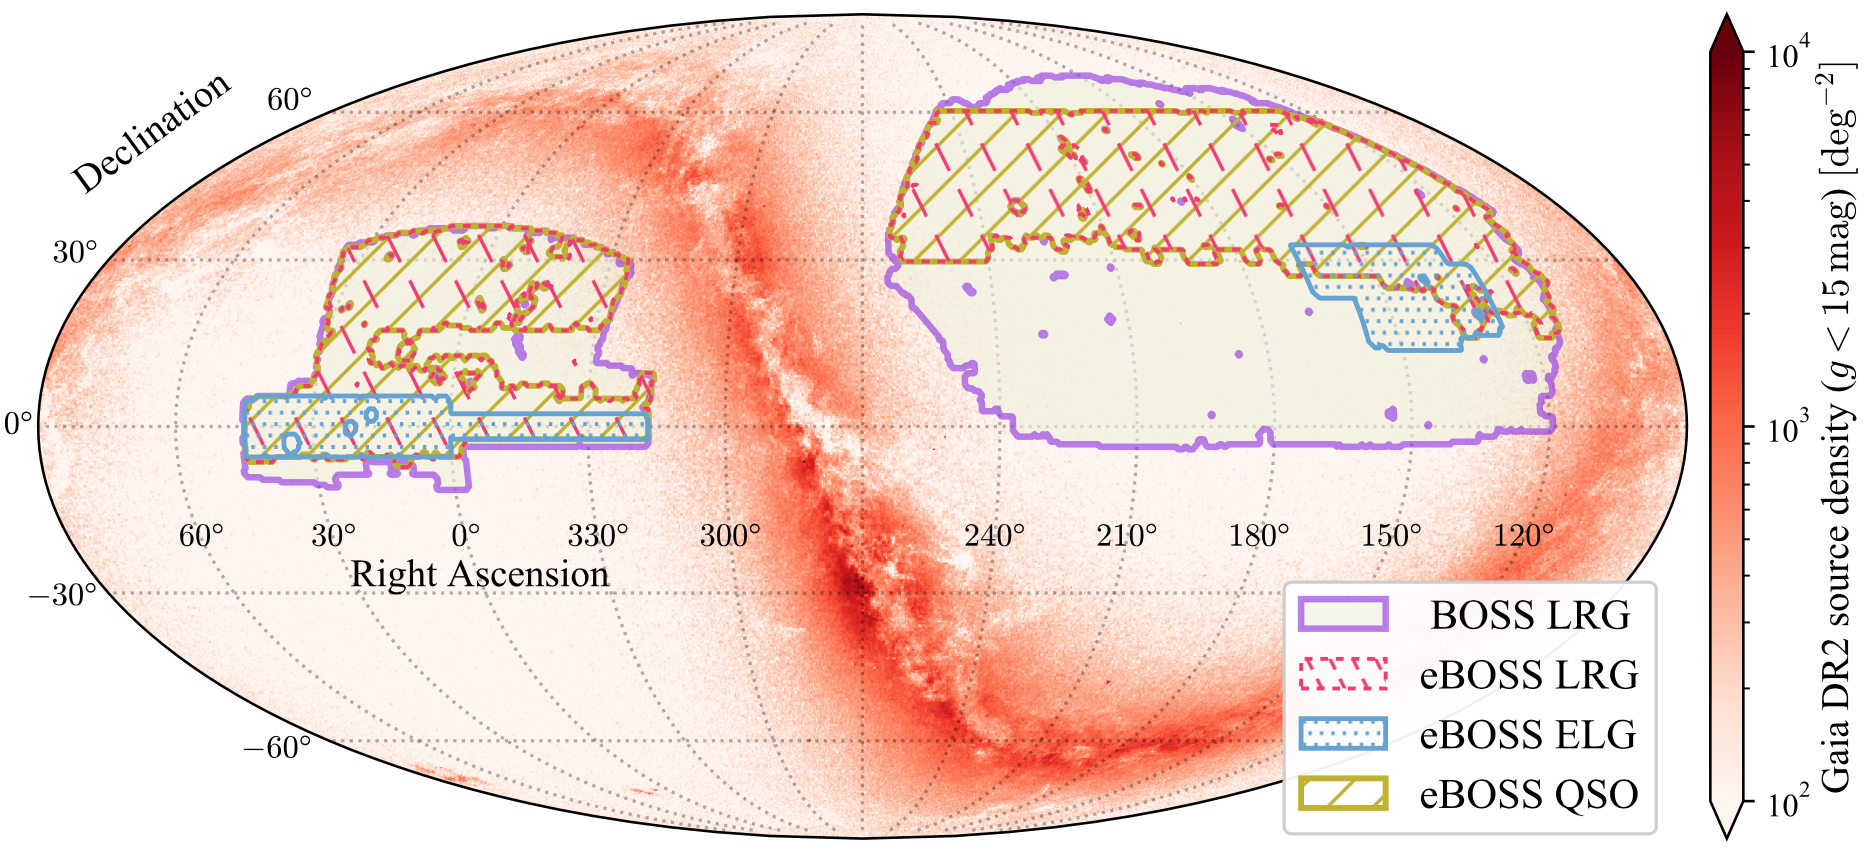
\includegraphics[width=0.9\textwidth]{fig/galaxies/eboss_footprint.png}
    \caption{ The DR16 footprint for each eBOSS tracer: Luminous Red Galaxies (LRG), 
    Emission Line Galaxies (ELG) and quasars (QSO). The BOSS DR12 LRGs area is also shown, 
    as well as the density map of Gaia DR2 sources with $g < 15$ mag.
    Figure extracted from \cite{zhaoCompletedSDSSIVExtended2021}.} 
    \label{fig:eboss_footprint}
\end{figure}

Some targets cannot be observed due to 
its proximity to another observed target and the finite size of fibres, corresponding 
to 62 arcseconds in the sky. We refer to these events as \emph{fibre collisions}. 
Collisions might happen not only to pairs of galaxies, but to any group of targets with 
linking lengths smaller than 62 arcsec. Depending on the number of plates observing 
a giving sector, some collisions might be solved but the missing ones  
impact the measured clustering on small scales if not corrected. 
While there are several methods to solve collisions 
(\cite{guoNewMethodCorrect2012, bianchiUnbiasedClusteringEstimation2017}),
we used the simplest up-weighting technique, where the nearest observed galaxy 
is up-weighted by the number of non-observed targets within the collision group. 
This assumes that non-observed targets are also galaxies of the same target type and 
that they are physically close (angularly and radially) to the observed ones.
On scales above a few \hmpc, this simple correction is a good approximation. 

Two additional sets of weights are defined to correct for spurious density 
fluctuations contaminating cosmological fluctuations in which we are interested. 
These weights could be applied to randoms but we chose to apply these to the 
galaxy themselves. 

The first set of weights corrects for angular fluctuations caused 
by correlations between galaxy number density and photometry-related quantities,
such as Galactic extinction, stellar density, imaging depth or sky flux.
They are commonly referred to as \emph{photometric weights}. 
Figure~\ref{fig:photo_systematics_lrg} displays these correlations 
for the LRG sample both before and after applying correction weights. 
For the analysis of eBOSS DR16 LRGs, I have 
implemented\footnote{\url{https://github.com/julianbautista/eboss_clustering/blob/master/python/systematic_fitter.py}} 
a multi-dimension 
linear regression that assumes these correlations are linear and 
accounts for the fact that some photometric quantities are correlated between themselves 
(e.g., stellar density and Galactic extinction).
This multi-linear method is based on work described in \cite{prakashSDSSIVExtendedBaryon2016}.
Of course, more advanced methods have been developed since then, based on 
machine learning algorithms 
(\cite{rezaieImprovingGalaxyClustering2020, chaussidonAngularClusteringProperties2021}).
It is important to evaluate the performance of these algorithms with mock catalogues
where we add artificial contamination 
and quantify how well we recover the initial raw power spectrum after correcting for them. 
There is a risk of overfitting and removing some large-scale cosmological modes which 
can be harmful for clustering analysis, particularly those aiming at measuring 
primordial non-Gaussianity 
(\cite{rezaiePrimordialNonGaussianityCompleted2021, muellerClusteringGalaxiesCompleted2021}).

\begin{figure}
    \centering 
    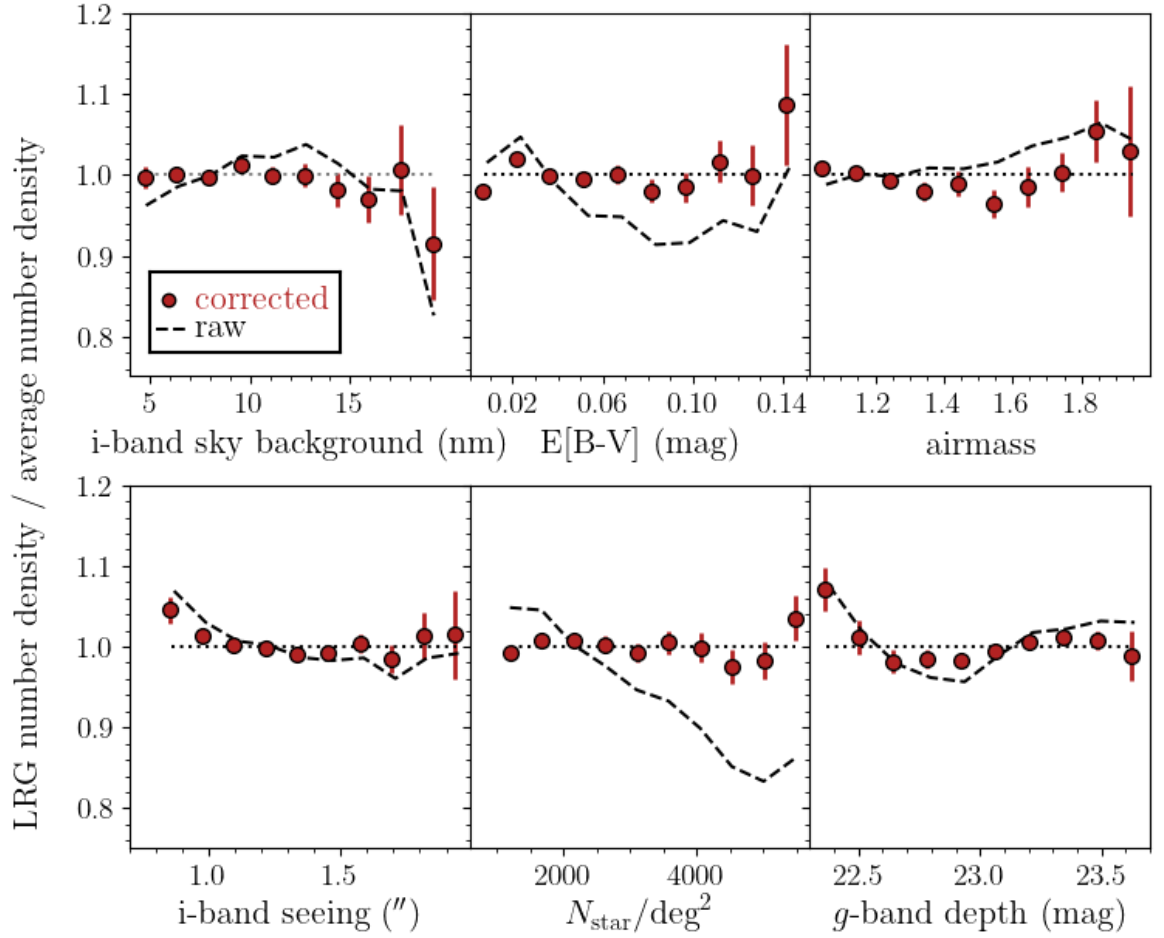
\includegraphics[width=0.7\textwidth]{fig/galaxies/photometric_weights_lrg.png}
    \caption{ Fluctuations in the angular LRG density as a function of 
    various imaging properties and Galactic foregrounds. 
    The dashed curves show these fluctuations before any correction 
    while red points show the result of applying a linear correction for 
    stellar density and Galactic extinction. 
    Figure extracted from \cite{rossCompletedSDSSIVExtended2020}.} 
    \label{fig:photo_systematics_lrg}
\end{figure}

The second set of weights corrects for the so-called \emph{redshift failures}, 
which are spectra with low signal-to-noise ratio (S/N)
not yielding a statistically significant redshift measurement. 
If redshift failures were randomly distributed across the sky, 
they would not introduce any particular bias to the clustering. 
However, given the particular configuration and throughput of the SDSS spectrographs, 
these failures imprint a pattern in the sky which contaminates clustering. 
The left panel of Figure~\ref{fig:eboss_zfailures} displays the average failure rate 
of eBOSS LRGs as a function of position in the focal plane. 
This pattern is due to the fact that fibres at the side edges of the focal plane 
transport light to the edges of the CCDs which have a lower-than-average throughput. 
The right panel of Figure~\ref{fig:eboss_zfailures} shows the 
dependency of the average redshift failure rate as a function of the signal-to-noise
ratio of the observation\footnote{The signal-to-noise ratio of an observation was 
defined internally as a function of the signal-to-noise ratio of all observed 
spectra and their magnitudes.}.
When modelling these dependencies of failure rates with S/N (or fibre number or focal plane
position), one can correct these spurious fluctuations by assigning a weight 
inversely proportional to the modelled rate. 
These \emph{redshift-failure weights} are assigned to the 
galaxies with confident redshift measurements, to compensate for the eventual 
non-confident ones at the same location in the focal plane. 

\begin{figure}
    \centering 
    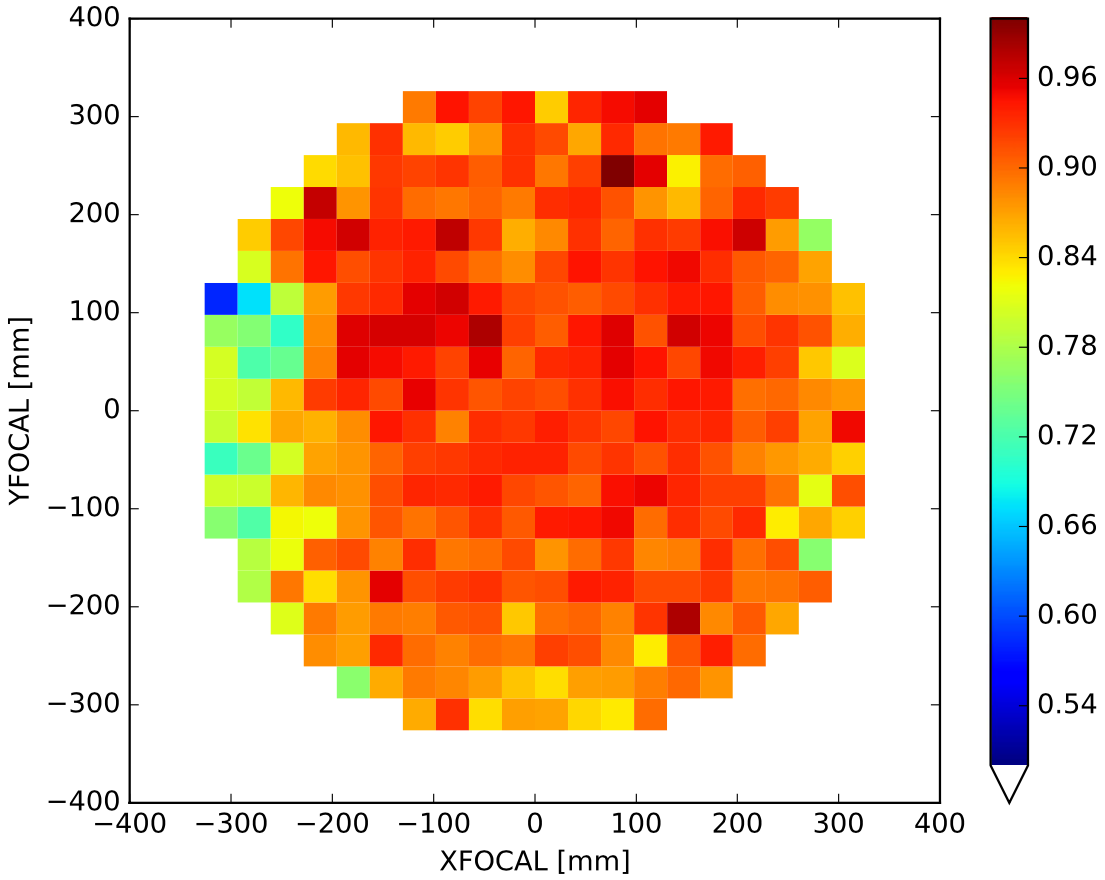
\includegraphics[width=0.49\textwidth]{fig/galaxies/eboss_z_failures_focalplane.png}
    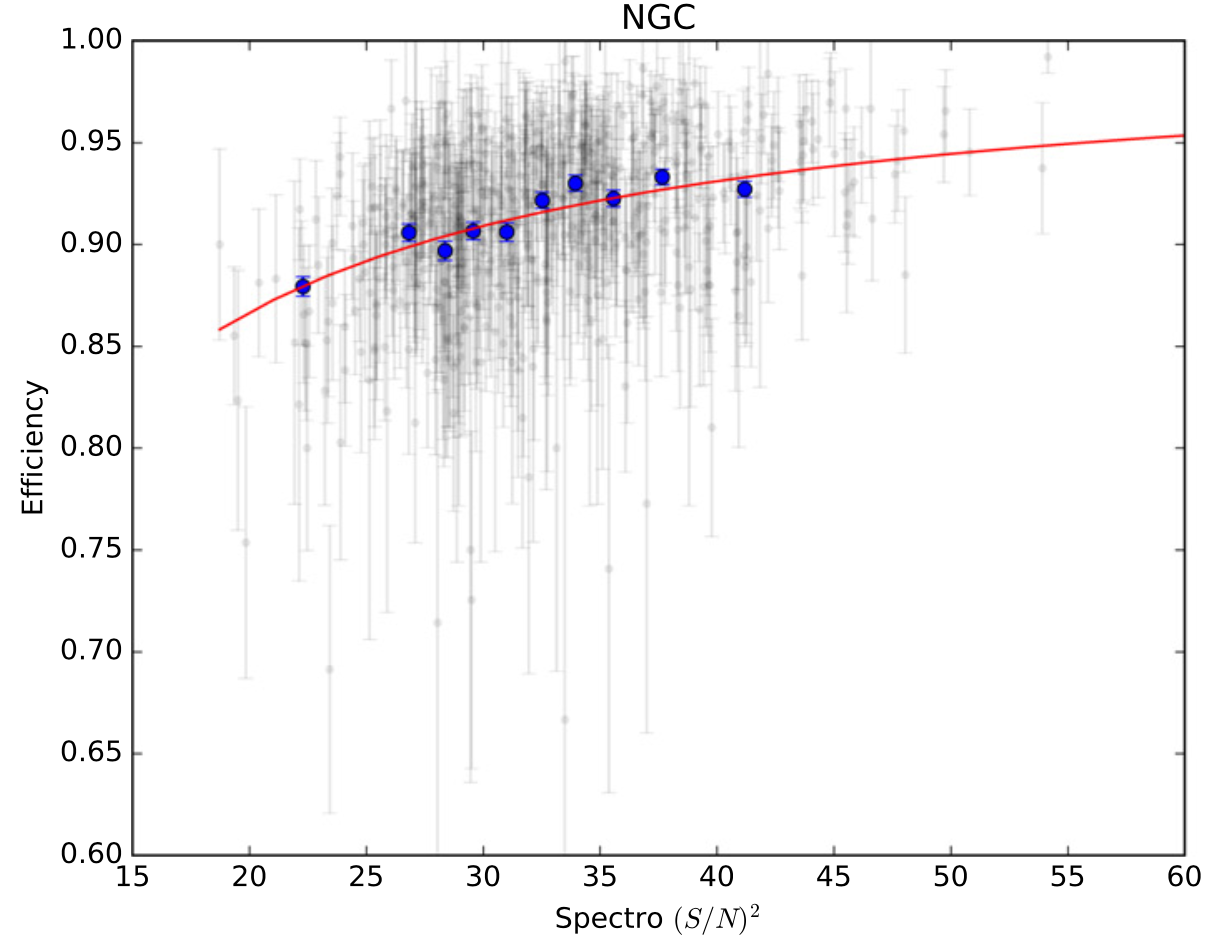
\includegraphics[width=0.49\textwidth]{fig/galaxies/eboss_z_failures_sn.png}
    \caption{ 
        Average redshift efficiency as a function of physical position of the optical 
        fiber in the focal plane (left panel) and as a function of the observation
        signal-to-noise squared (right panel).  
        The left panel shows how redshift-failures imprint a pattern on the sky 
        and therfore must be corrected. The right panel shows the underlying reason 
        for the failures. The model (red line) is used to compute correction weights.
    Figures extracted from \cite{bautistaSDSSIVExtendedBaryon2018}.} 
    \label{fig:eboss_zfailures}
\end{figure}

Once all galaxies have their correction weights (fibre collision, photometric and 
redshift-failure) and the randoms are corrected by fibre completeness, 
it is time to compute the radial selection function. 
The idea is to assign redshifts to randoms 
such that they follow the same redshift distribution as the galaxies. 
The redshift distribution is often quantified by the comoving galaxy (weighted)
number density $\bar{n}(z)$. 
Figure~\ref{fig:eboss_z_distrib} shows the comoving density of eBOSS tracers 
as a function of redshift. 
For randoms to match this distribution, we randomly assign galaxy 
redshifts to each random, with repetition. Another possibility would be to 
fit some smooth function over the observed $\bar{n}(z)$ and draw random redshifts
from the resulting model. All these methods introduce the so called 
\emph{radial integral constraint}, i.e., the fact that the observed $\bar{n}(z)$ is 
not the true ensemble averaged function of the Universe, but derived from the 
volume-limited realisation that we observe. 
The impact on clustering of the radial integral constraint is 
inversely proportional to the area of the footprint
(\cite{demattiaIntegralConstraintsSpectroscopic2019}) and it is significant 
for surveys such as the eBOSS ELG (see Figure~\ref{fig:eboss_footprint} and 
\cite{tamoneCompletedSDSSIVExtended2020, demattiaCompletedSDSSIVExtended2021}). 


\begin{figure}
    \centering 
    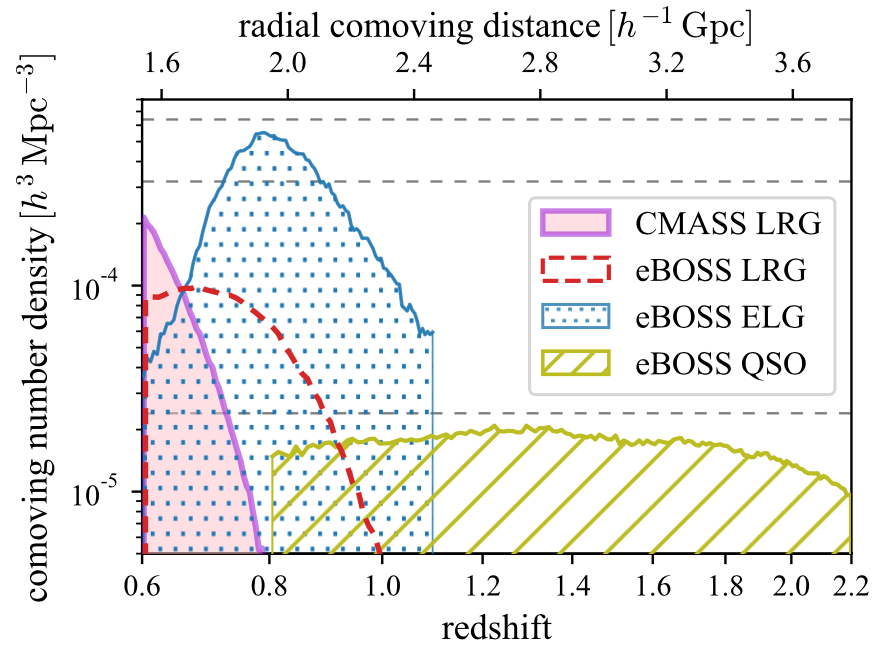
\includegraphics[width=0.6\textwidth]{fig/galaxies/eboss_z_distribution.png}
    \caption{ The weighted comoving number densities $\bar{n}(z)$ of eBOSS DR16 tracers
    and BOSS DR12 CMASS LRGs, with all the photometric and spectroscopic
    systematic weights included. 
    The comoving distances and volumes are computed assuming a flat-$\Lambda$CDM 
    cosmology with $\Omega_m = 0.31$. 
    %The three horizontal dashed lines show the number densities of the cubic LRG, ELG, and QSO    
    %EZmockcatalogues,i.e. $3.2 \times 10^{-4}$, $6.4 \times 10^{-4}$, and $2.4 \times 10^{-5} h^3 \text{Mpc}^{-3}$, respectively.
    Figure extracted from \cite{zhaoCompletedSDSSIVExtended2021}.} 
    \label{fig:eboss_z_distrib}
\end{figure}

The final step of the catalogue production consists in adding an additional set of weights 
to galaxies that optimise the signal-to-noise ratio of clustering measurements 
when the redshift distribution is not uniform. These weights were first introduced 
by \cite{feldmanPowerSpectrumAnalysisThreedimensional1994} and have been applied 
to all clustering analysis ever since. They are commonly referred to as 
\emph{FKP weights} and can be written for a galaxy $i$ as
\begin{equation}
    w_\text{i, FKP} = \frac{1}{1 + \bar{n}(z_i)P_0}
\end{equation}
where $P_0$ is a rough value of the power spectrum of the tracers at some 
particular scale of choice, usually BAO scales for large-scale clustering measurements.
For eBOSS analyses, we chose a scale of $k \sim 0.1 h\, \text{Mpc}^{-1}$ for which 
$P_0 = 10000 h^{-3}\text{Mpc}^{3}$ for LRGs, 
$P_0 = 4000 h^{-3}\text{Mpc}^{3}$ for ELGs and 
$P_0 = 6000 h^{-3} \text{Mpc}^{3}$ for QSOs. 

In summary, the random catalogue describes the angular and radial selection functions
of the galaxy survey. 
Each random has a weight $w_r = w_\text{comp} w_\text{FKP}$, where $w_\text{comp}$ accounts
the spectroscopic completeness of targets and $w_\text{FKP}$ are optimal weights for clustering. 
Each galaxy has a weight given by $w_g = w_\text{col} w_\text{photo} w_\text{fail} w_\text{FKP}$,
where $w_\text{col}$ accouns for fibre collisions, $w_\text{photo}$ corrects fluctuations caused 
by photometry and $w_\text{fail}$ corrects redshift failures. 
These weights are employed when computing correlation functions 
or power spectra (see~\ref{galaxies:clustering}).

\section{Reconstruction of linear density field} 
\label{galaxies:reconstruction}

Bulk motions of galaxies on scales of tens of Mpc impact their two-point statistics, 
acting as a smoothing of the clustering (\cite{eisensteinRobustnessAcousticScale2007}).  
In particular, these motions smooth/broaden the BAO peak, 
reducing the precision on our measurement of its position. 
In the past decades, several methods have been proposed to reconstruct
the linear density field and remove these bulk motions from a galaxy survey,
therefore sharpening the BAO peak.
These methods are referred to as \emph{reconstruction} methods. 
Reconstruction is now an essential part of standard BAO measurements from galaxy surveys,
since they improve significantly their precision. 

The simplest form of reconstruction is based on a theoretical relationship between 
the galaxy density field on large scales (our observable) and the displacement field connecting 
the observed field (Eulerian frame) to its past version (Lagrangian frame). 
Lagrangian perturbation theory (LPT) can predict these displacements 
(see \cite{bernardeauLargeScaleStructureUniverse2002} for a review). 
To first order, the relation between displacements and density is linear 
(\cite{zeldovichGravitationalInstabilityApproximate1970}). From the observed 
density field in our survey, we can compute the corresponding linear displacements
and move galaxies back. Since we want to ``move'' the density field, we also move randoms 
by the same displacements. 
This procedure successfully removes most of the broadening of the BAO peak
(\cite{nusserTracingLargeScaleFluctuations1992, eisensteinImprovingCosmologicalDistance2007}).
The first order LPT reconstruction is often called \emph{Zeldovich reconstruction}. 
Extending to second order LPT does not improve BAO reconstruction significantly 
(\cite{seoHighprecisionPredictionsAcoustic2010}) but it helps on recovering the 
velocity field (\cite{kitauraEstimatingCosmicVelocity2012}).
Zeldovich reconstruction has been used in all BAO measurements from SDSS (BOSS and eBOSS).
I implemented a python version\footnote{\url{https://github.com/julianbautista/eboss_clustering/}} of 
the Zeldovich reconstruction that uses Fast Fourier Transforms while accounting for the 
large angle effects 
(\cite{burdenEfficientReconstructionLinear2014, burdenReconstructionFourierSpace2015}). 
Alternatively, displacements can be computed 
in configuration space using finite difference approximations (\cite{padmanabhanCentDistance352012})
though these are slower and less precise than iterative FFTs. 

Since we do not observe the actual density of matter, a bias relation between galaxy number density 
and matter density has to be assumed in reconstruction. Usually we assume a linear bias relation, where the 
bias value is estimated from the clustering of the standard galaxy catalogue. 
This is a reasonable approximation 
since reconstruction uses fluctuations on scales larger than $\sim 15$\hmpc. 
It is also possible to remove linear redshifts-space distortions, 
by assuming a value for the growth-rate of structures $f$
(see section~\ref{intro:probes:rsd}) used to convert the displacements into velocities.
The radial components of the estimated velocities are then removed from each galaxy.  
Therefore, the clustering of reconstructed catalogues depend on the fiducial values of bias and $f$, 
but less on the distance-redshift relation (\cite{carterImpactFiducialCosmology2020}). 

There are other backward reconstruction techniques such as those based on the least action principle (LAP).
First proposed by \cite{peeblesTracingGalaxyOrbits1989}, it was extended to cosmological applications 
by \cite{nusserLeastActionPrinciple2000, sarpaBAOReconstructionSwift2019}. 
\cite{sarpaExtendedFastAction2021} applied it for the BAO measurement of the BOSS DR12 galaxy sample. 

Reconstruction is essential to improve the precision on BAO measurements. However, 
due to imperfections in recovering the true initial conditions, 
reconstruction has not yet been used in attempts to derive cosmological 
constraints from the full-shape of the reconstructed two-point statistics.
Therefore, analysis of redshift-space distortions are based on the non reconstructed 
clustering (see section~\ref{galaxies:rsd}).  

\section{Mock catalogues}
\label{galaxies:mocks}

An important limitation in cosmology is that we only have a single realisation of our Universe. 
Therefore simulations are an essential tool to overcome this limitation. 

We can recognise two types of simulations mainly used in cosmology. First, 
n-body simulations (eventually including gas) solve numerically for the formation of structures
and are computationally expensive. They focus on the fully non-linear aspects and require a 
higher resolution setting, preventing them to simulate very large volumes or producing numerous 
realisations. N-body simulations are still the baseline for tests of perturbation theory models.
See \cite{anguloLargescaleDarkMatter2022} for a review on cosmological n-body simulations.  
The second type of simulations are the so-called \emph{mock catalogues} or simply \emph{mocks}. 
They are lower resolution and do not fully describe the non-linear clustering but they are 
faster to produce both in large volumes and in large number of realisations.
Their are key for the understanding of biases in best-fitted quantities and on their uncertainties 
in clustering analyses. 
Given the large number of realisations, mocks have been the most reliable method to estimate 
covariance matrices of clustering measurements. 
Also, mocks are used to study the impact of observational systematic effects on our 
measurements. 
All previous cosmological measurements from galaxy surveys have associated sets of 
n-body simulations and mock catalogues. I will describe the example I was involved in, 
the case of \textsc{EZmocks} produced for the eBOSS DR16 clustering measurements. 

A set of 1000 \textsc{EZmock} realisations of the eBOSS survey were produced for three tracers:
LRGs, ELGs and QSOs. 
They are fully described in \cite{zhaoCompletedSDSSIVExtended2021}. 
These mocks employ an effective Zeldovich approximation to evolve 
the density field in longer time steps (\cite{chuangEZmocksExtendingZel2015}). 
By construction, these mocks match the large-scale clustering 
of the target data sample, including 2 and 3-point statistics. 
They have some extra free parameters to simulate a biased galaxy sample and non-linear motions on small-scales.  
The eBOSS \textsc{EZmocks} also include light-cone effects produced by interpolating boxes
at different redshifts. 

The last step in the production of \textsc{EZmocks} was the addition of systematic effects. 
I was responsible of implementing all known observational effects from the data onto the mocks. 
A simple script\footnote{\url{https://github.com/julianbautista/eboss_clustering/blob/master/bin/ezmocks_add_systematics.py}}
gathers the information from the real catalogues and simulates fibre collisions, spurious 
fluctuations caused by photometry and spectroscopy. 
These contaminated mocks are then corrected using the same algorithms as for the real data, 
as described in section~\ref{galaxies:catalogue}. The clustering before and after adding 
those effects is extensively compared to real data (\cite{zhaoCompletedSDSSIVExtended2021}) 
and the agreement is found to be excellent on the scales of interest for BAO and RSD measurements. 



\section{From catalogues to clustering estimates}
\label{galaxies:clustering}

Once the catalogue of galaxies and the associated random catalogue are ready, 
any statistical quantity can be computed, such as $n$-point statistics. 
As discussed in section~\ref{intro:lss}, these statistics can be computed 
in either configuration space or Fourier space. 
This section describes how to obtain 2-point function estimates, 
in both spaces, which are the statistics I worked with. 

\subsection{Correlation function}
\label{galaxies:clustering:correlation_function}

The estimate of the correlation function $\xi(\vec{r})$ is based on counting pairs of galaxies 
in bins of separation $\vec{r}$ and comparing it to same numbers obtained from the random catalogue. 
For the estimator we use, there is no need to calculate galaxy number densities $n(\vec{x})$  
or overdensities $\delta_n(\vec{x})$ in some mesh. To optimise the variance of the estimator 
while keeping it unbiased, \cite{landyBiasVarianceAngular1993} proposed to include the cross-pairs  
between galaxies and randoms in the estimator, yielding:
\begin{equation}
 \xi(\vec{r}_i) = \frac{DD(\vec{r}_i) - 2DR(\vec{r}_i)}{RR(\vec{r}_i)} + 1,
 \label{eq:landy-szalay}
\end{equation}
where $DD(\vec{r}_i)$ (or $RR(\vec{r}_i)$) are the normalised paircounts between galaxies (or randoms) 
at bin $i$ corresponding to separation $\vec{r}_i$, 
$DR(\vec{r}_i)$ is the normalised cross-paircounts between galaxies and randoms. 
The normalisation of the paircounts is given by the total number of unique pairs in the catalogue, 
i.e., $N(N-1)/2$ if the catalogue contains $N$ galaxies or $N_g N_r$ for the cross pairs. 
When using weights as described in section~\ref{galaxies:catalogue}, nothing changes except 
that each pair of galaxies (or randoms) are weighted as $w_{ij} = w_i w_j$, where $w_i, w_j$ are the 
weights of each element of the pair. 

More recently, new ways to account for fibre collisions 
or incompleteness have been proposed 
(\cite{bianchiUnbiasedClusteringEstimation2017, percivalUsingAngularPair2017}) where each pair 
of galaxies would have a weight $w_{ij} \neq w_i w_j$, i.e., not a product of individual weights. 
This makes the calculation slighly slower since these weights have to be defined for each pair. 
These new estimators were first used with the eBOSS tracers
(\cite{mohammadCompletedSDSSIVExtended2020}) and are currently being employed within DESI. 

The estimator in Eq.~\ref{eq:landy-szalay} changes slightly when dealing with catalogues 
resulting from reconstruction algorithms,
where both galaxies and randoms are shifted in order to reduce the impact of bulk motions 
(see section~\ref{galaxies:reconstruction}). 
The Landy-Szalay estimator is now written as  
\begin{equation}
    \xi^\text{recon}(\vec{r}_i) = \frac{DD(\vec{r}_i) - 2DS(\vec{r}_i) + SS(\vec{r}_i)}{RR(\vec{r}_i)},
    \label{eq:landy-szalay-recon}
\end{equation}
where $S$ represents the shifted random catalogue and the $R$ is the usual random catalogue as before. 
See \cite{padmanabhanReconstructingBaryonOscillations2009, padmanabhanCentDistance352012} 
for a detailed derivation of this estimator. 

Most analyses of the two-point correlation function do not use the full $\xi(\vec{r}_i)$,
where $\vec{r}_i$ are bins in 2D separations such as bins in $(\rpara, \rperp)$ or $(r, \mu_r)$.
Most analysis further compress the estimated correlation function into a new basis with fewer 
degrees of freedom. Some analyses uses the correlation function 
\emph{wedges} $\xi_{\mu_{r1}, \mu_{r}}(r)$, which are 
averages of $\xi$ over $\mu_{r1} < \mu < \mu_{r2}$, as already discussed in section~\ref{forests:bao:correlations}. 
Other analyses, such as the one described in this chapter, decompose $\xi$ into a basis of 
Legendre polynomials $L_\ell(\mu_r)$ such that $\xi(r, \mu_r) = \sum_\ell \xi_\ell(r) L_\ell(\mu_r)$, 
where $\xi_\ell(r)$ are the correlation function \emph{multipoles}. 
Usually two or three wedges or multipoles are considered when comparing to clustering models.  

One of the most recent codes to compute correlation function accounting for all 
features described above is 
\textsc{pycorr}\footnote{\url{https://github.com/cosmodesi/pycorr}} 
which is being currently developed for DESI.

\subsection{Power spectrum}
\label{galaxies:clustering:power_spectrum}

The power spectrum is the analogous of the correlation function in Fourier space. 
It requires a Fourier Transform of the galaxy overdensity field, which introduces 
some effects that have to be correctly taken into account when fitting for clustering models. 
The power spectrum estimation is based on work by 
\cite{feldmanPowerSpectrumAnalysisThreedimensional1994,
bianchiMeasuringLineofsightdependentFourierspace2015,
handOptimalFFTbasedAnisotropic2017} and it is shortly described here. 

The first step is to assign galaxies and randoms into a three-dimensional mesh, 
defining an ``overdensity'' function $F(\vec{x}_i)$ as 
\begin{equation}
    F(\vec{x}_i) =  n(\vec{x}_i) - \alpha n_\text{rand}(\vec{x}_i),
    \label{eq:overdensity_fourier}
\end{equation}
where $n_\text{rand}$ are the \emph{weighted} number density of galaxies and randoms in voxel centered at $\vec{x}_i$, 
$\alpha$ is the ratio of the total weighted number of galaxies to the total weighted number of randoms. 
The field $F(\vec{x})$ is also kwown as the FKP field. 

The field $F(\vec{x})$ can be Fourier transformed numerically using Fast Fourier Transform (FFT) 
algorithms. The power spectrum would be defined as the absolute value squared of this field. 
Power spectrum \emph{multipoles} are commonly 
used, as it was the case in configuration space. 
They can be expressed as: 
\begin{equation}
 P_\ell(k) = \frac{1}{I_{22}} \left[ (2\ell+1) \left\langle F_0(\vec{k})F_\ell(-\vec{k}) \right\rangle_{V_k} - (1+\alpha)I_{12} \delta_{0\ell} \right]
 \label{eq:power_spectrum_multipoles}
\end{equation}
where the brakets $\langle \cdot \rangle$ indicate average over spherical shells in k-space with radius $|\vec{k}|$, 
$F_\ell(\vec{k})$ are the overdensity multipoles in k-space given by 
\begin{equation}
    F_\ell(\vec{k}) = \int \text{d}^3x F(\vec{x}) \text{e}^{i \vec{k}\cdot \vec{r}} L_\ell( \hat{k} \cdot \hat{x}), 
\end{equation}
and the normalisation factors $I_{ab}$ are defined as 
\begin{equation}
 I_{ab} \equiv \int \text{d}^3 x [n(\vec{x})]^a [w_\text{FKP}(\vec{x})]^b. 
 \label{eq:normalisation_power_spectrum}
\end{equation}

The first term in Eq.~\ref{eq:power_spectrum_multipoles} is the usual term defining the power spectrum, i.e., 
the square of the absolute value of Fourier fluctuations, while the second term is the so called \emph{shot-noise} 
and only affects the power spectrum monopole. 

Since we use Fourier transforms which rely on periodic boundary conditions, the mesh used to compute $F(\vec{x})$
has to be large enough to encompass the survey volume with some padding around it. 
Also, because of the assumption of periodicity, the estimated power spectra will be convolved by the window/selection function of the survey.
This window has to be correctly computed using the randoms and 
it is a key ingredient to be accounted for when modelling the clustering. 

Since we use numerical FFTs, the resolution of the mesh defines the scales being probed. 
If the mesh has a total comoving size of $L$ on a side and has $N$ voxels on a side, 
the fundamental mode is given by $k_F = \pi/L$ while the highest (or Nyquist) frequency is $k_\text{Ny} = \pi N/L$. 
Typically meshes with 512 or 1024 voxels on a side are sufficient to cover the scales of interest 
for BAO or RSD analyses in current survey volumes, $0.01 < k < 0.30 (\text{Mpc}/h)^{-1}$. 

The estimated power spectra are also affected by the discreteness nature of the mesh on scales close 
the Nyquist frequency. The assignement of galaxies to the mesh can be optimised to reduce those effects. 
Also, interlacing techniques can also further reduce mesh effects. 
These effects and proposed solutions are described in detail in \cite{sefusattiAccurateEstimatorsCorrelation2016}
and are implemented in the package \textsc{nbodykit}\footnote{\url{https://nbodykit.readthedocs.io/}}
or \textsc{pypower}\footnote{\url{https://github.com/cosmodesi/pypower}}. 

\subsection{The clustering of eBOSS DR16 LRGs}
\label{galaxies:clustering:eboss_dr16_lrgs}

Figure~\ref{fig:LRG_data_ezmock_correlations_prerec} and \ref{fig:LRG_data_ezmock_correlations_postrec}
show the power spectrum $P_\ell(k)$ and correlation function $\xi_\ell(r)$ multipoles for $\ell = 0, 2, 4$
for the combined sample of BOSS DR12 and eBOSS DR16 luminous red galaxies and their respective \textsc{EZmock}
catalogues. Figure~\ref{fig:LRG_data_ezmock_correlations_prerec} shows results from standard catalogues while 
Figure~\ref{fig:LRG_data_ezmock_correlations_postrec} displays results from reconstructed catalogues. 

\begin{figure}
    \centering
    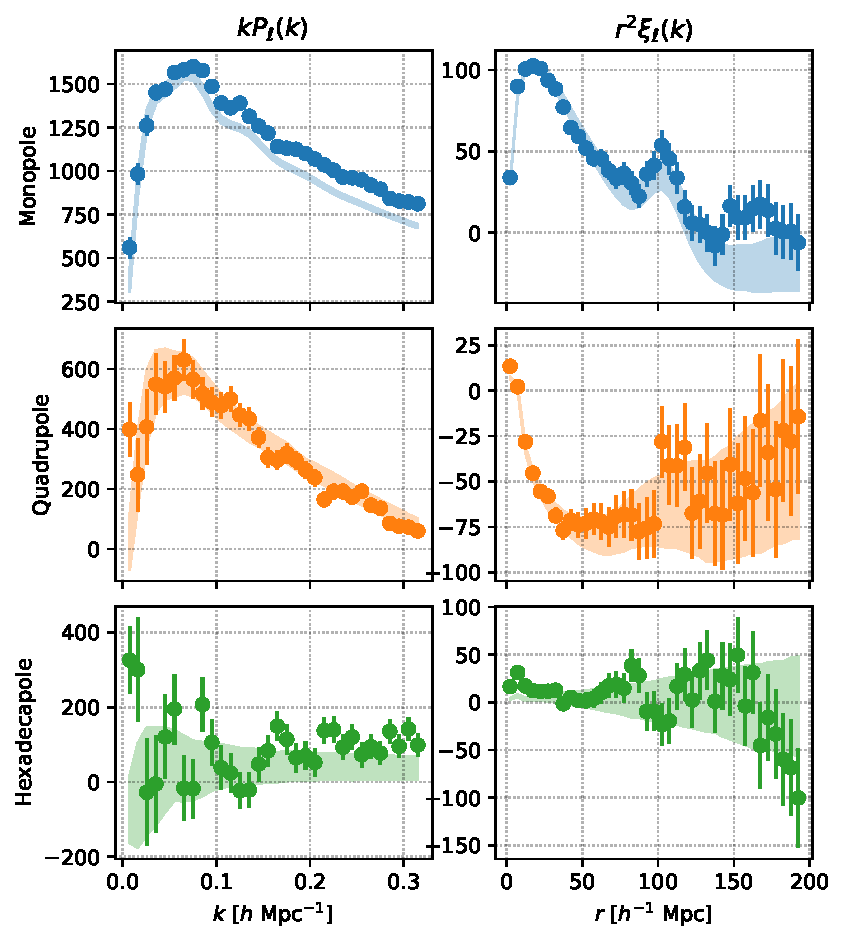
\includegraphics[width=0.8\textwidth]{fig/galaxies/DR16LRG_data_ezmock_prerecon.pdf}
    \caption{Pre-reconstruction multipoles of the two-point statistics for the combination of BOSS DR12 and 
    eBOSS DR16 luminous red galaxies. Left panels contain the power spectrum multipoles (scaled by $k$) 
    and right panels the correlation function multipoles (scaled by $r^2$). 
    Points with errorbars are real data while shaded regions show the mean and standard deviation 
    of 1000 realisations of \textsc{EZmocks}. 
    }
    \label{fig:LRG_data_ezmock_correlations_prerec}
\end{figure}

\begin{figure}
    \centering
    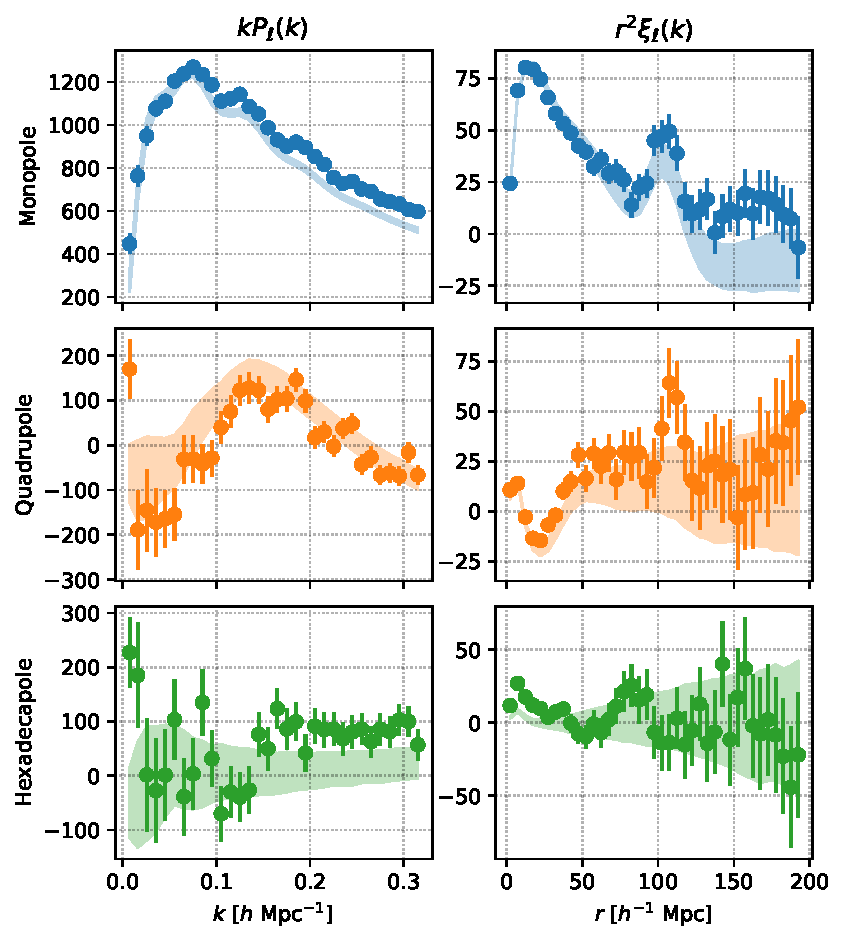
\includegraphics[width=0.8\textwidth]{fig/galaxies/DR16LRG_data_ezmock_postrecon.pdf}
    \caption{Same as Figure~\ref{fig:LRG_data_ezmock_correlations_prerec} but for reconstructed 
    catalogues. We used the Zeldovich reconstruction method with removal of redshift-space distortions. 
    The BAO features are more proeminent and the quadrupole is significantly reduced compared 
    to results with the standard catalogues.    
    }
    \label{fig:LRG_data_ezmock_correlations_postrec}
\end{figure}

The uncertainties on our measurements of $P_\ell$ and $\xi_\ell$ were derived by measuring the 
same statistics on the full sample of 1000 realisations of \textsc{EZmocks}. By reproducing with 
high fidelity the observational features and systematic effects, the covariance matrix obtained 
with mocks should account for the extra scatter induced by them. However on small scales the 
clustering of the mocks is not accurate compared to real data or to more realistic n-body simulations. 
Figure~\ref{fig:covariance_ezmock} shows the resulting covariance matrices normalised by the 
diagonal elements (correlation coefficients). We see how power spectra multipoles are generally 
less correlated than correlation function multipoles. Reconstruction also helps reducing these 
correlations. Also shown are the cross-covariance between Fourier space and configuration space 
measurements, which will be discussed in section~\ref{galaxies:joint}. As expected, these
two spaces are highly correlated since they originate from the same sample of galaxies and randoms. 

\begin{figure}
    \centering 
    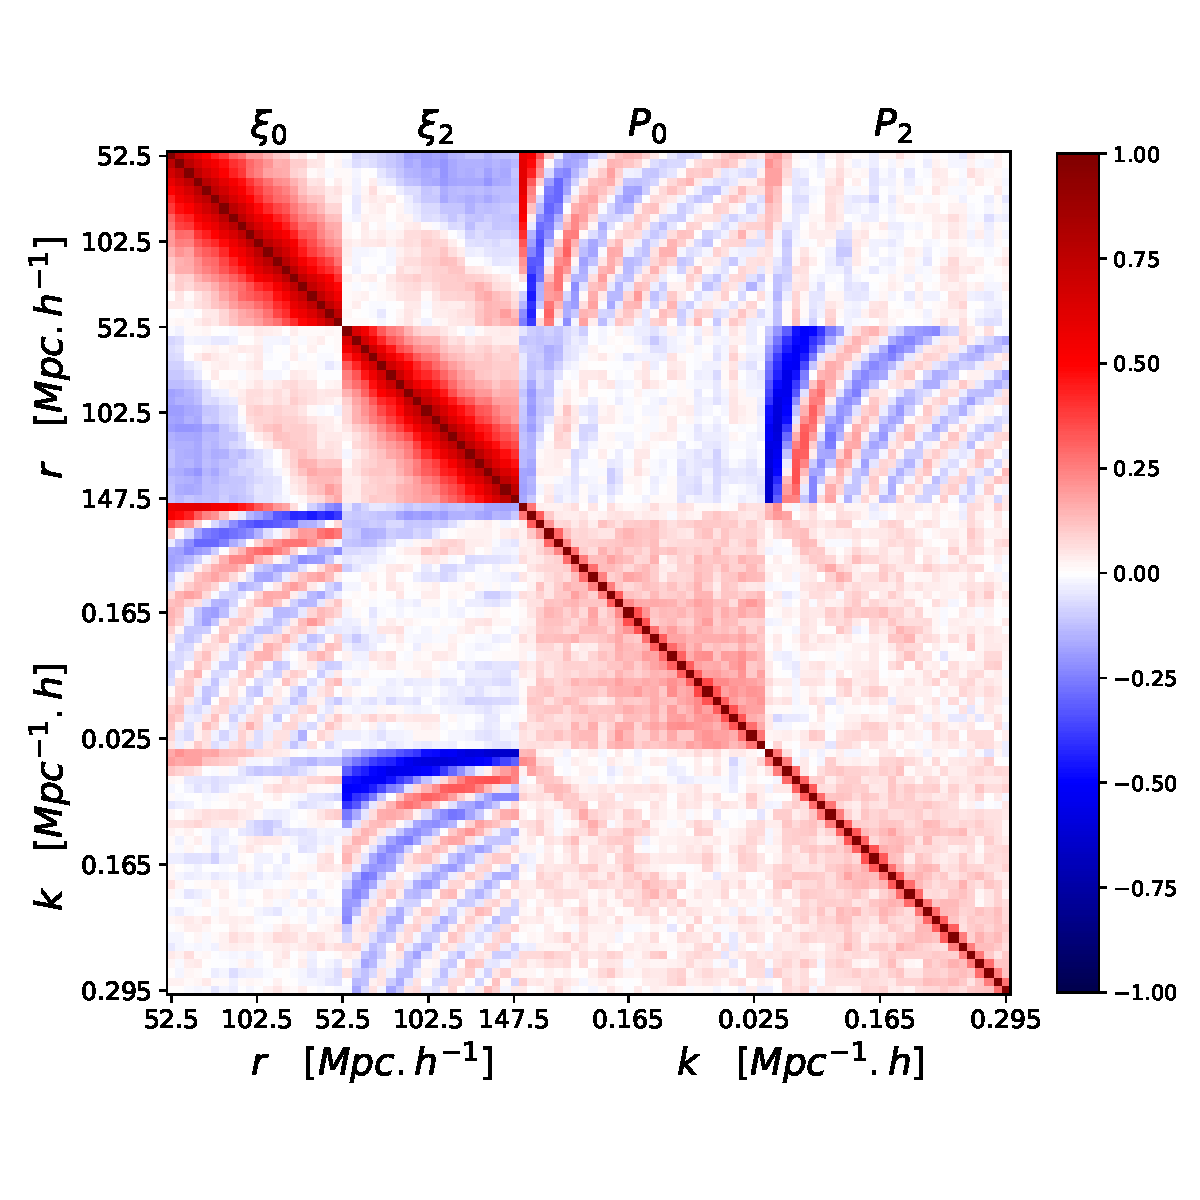
\includegraphics[width=0.49\textwidth]{fig/galaxies/covariance_prerecon.pdf}
    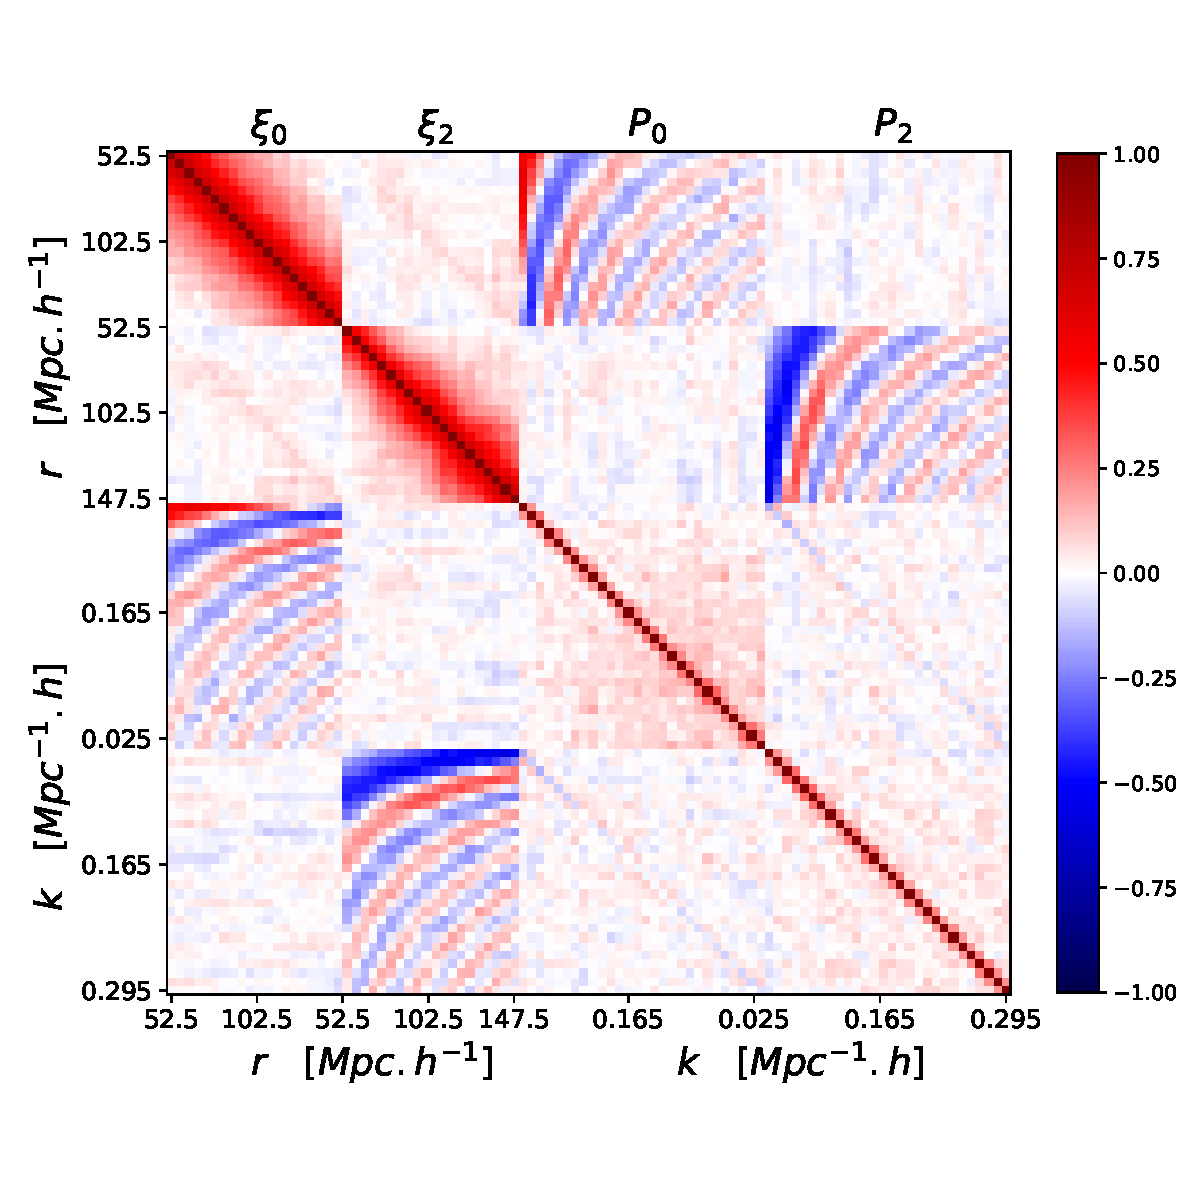
\includegraphics[width=0.49\textwidth]{fig/galaxies/covariance.pdf}
    \caption{Correlation coefficients from covariance matrices obtained from 1000 measurements
    of power spectrum and correlation function multipoles, $P_\ell$ and $\xi_\ell$ respectively,
    from \textsc{EZmocks} reproducing the combined BOSS DR12 and eBOSS DR16 LRG sample.
    Left panel shows results from the standard catalogues while the right panel 
    shows the results from Zeldovich reconstructed catalogues. 
    }
    \label{fig:covariance_ezmock}
\end{figure}


\section{Baryon acoustic oscillations}
\label{galaxies:bao}

The feature from baryon acoustic oscillations (BAO) is clearly visible 
as oscillations in the power spectrum multipoles and as a sharp peak 
in the correlation function multipoles 
(Figures~\ref{fig:LRG_data_ezmock_correlations_prerec} and 
\ref{fig:LRG_data_ezmock_correlations_postrec}). 
In this section I describe how we measure the BAO scale, which 
is used as a standard ruler in the study of the expansion of the Universe. 
The work is detailed further in 
\cite{bautistaCompletedSDSSIVExtended2021,
gil-marinCompletedSDSSIVExtended2020}.

The model used to fit BAO is based on the linear matter power spectrum with a simplified
treatment of bias, redshift-space distortions and non-linearities. 
It is basically the same model as used in the BAO measurements from 
\lya forests described in section~\ref{forests:bao:model} but without 
the treatment of metal absorption, high-column density systems and 
distortions which do not apply here. 
A linear bias and linear redshift-space distortions is assumed. 
The non-linearities that broaden the BAO peak are modelled by two 
Gaussian smoothing terms, one for radial separations and one for transverse separations. 
We also decompose the peak part from the smooth part of the model, 
scaling only the peak part by the dilation factors $\apara$ and $\aperp$, 
defined in Eqs.~\ref{eq:alpha_parallel} and \ref{eq:alpha_perp}.
The fit is performed in the space of multipoles instead of fitting for the 
full two-point statistics. Smooth power-laws of separation are added with free amplitudes 
in order to marginalise any potential information coming from 
the smooth part of the correlation function. 
To account for the removal of redshift-space distortions after reconstruction, 
an empirical damping term is added to the model, such that the linear RSD term 
$(1+\beta \mu^2)$ becomes $(1+ S(k) \beta \mu^2)$ where 
$S(k)\equiv 1- \text{e}^{-k^2\Sigma^2_\text{rec}/2}$ 
(\cite{seoModelingReconstructedBAO2016}). 

The methodology was tested with the sample of 1000 \textsc{EZmocks} 
and also an additional set of 84 \textsc{Nseries} n-body simulations 
(section~\ref{galaxies:mocks}). 
In principle, BAO is a feature on large enough scales 
such that testing the method on approximate mocks is sufficient, 
although we also looked at results on more realistic n-body simulaltions. 
In order to understand potential biases in best-fit BAO parameters, 
we fit for BAO on the average clustering of all available realisations 
for \textsc{EZmocks} and \textsc{Nseries} mocks,
effectively increasing the volume of the survey by a factor of 1000 and 84
respectively. Thanks to the large number of \textsc{EZmocks}, we 
were able to study the performance of our fitter statistically, 
by looking at the ensemble of 1000 individual BAO fits. 

Figure~\ref{fig:bao_bias_mocks} displays the results of fits 
to the mean clustering of mocks for 
catalogues pre- and post-reconstruction, also as a function of the 
fiducial choice for $\Omega_m^\text{fid}$ used in converting distances to redshifts. 
First we notice how biases are much smaller for reconstructed catalogues 
than standard ones, likely thanks to a better modelling of non-linearities 
affecting the BAO peak which are reduced in the reconstructed case. 
Second, uncertainties of reconstructed results 
are reduced relative to pre-reconstruction catalogues, 
showing the good performance of the method to remove 
bulk motions. 
Third, there is a very weak dependency of our results with the choice of
$\Omega_m^\text{fid}$, which is reassuring. 

\begin{figure}
    \centering 
    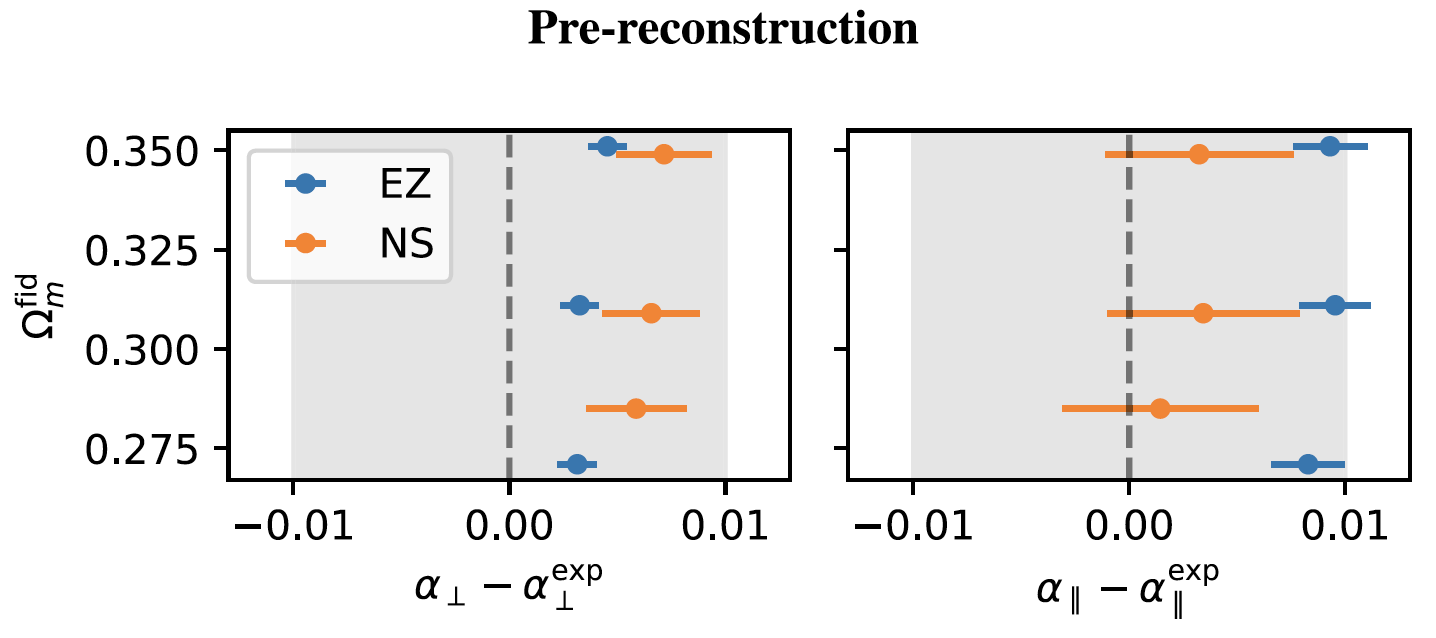
\includegraphics[width=0.49\textwidth]{fig/galaxies/bao_bias_prerecon.png}
    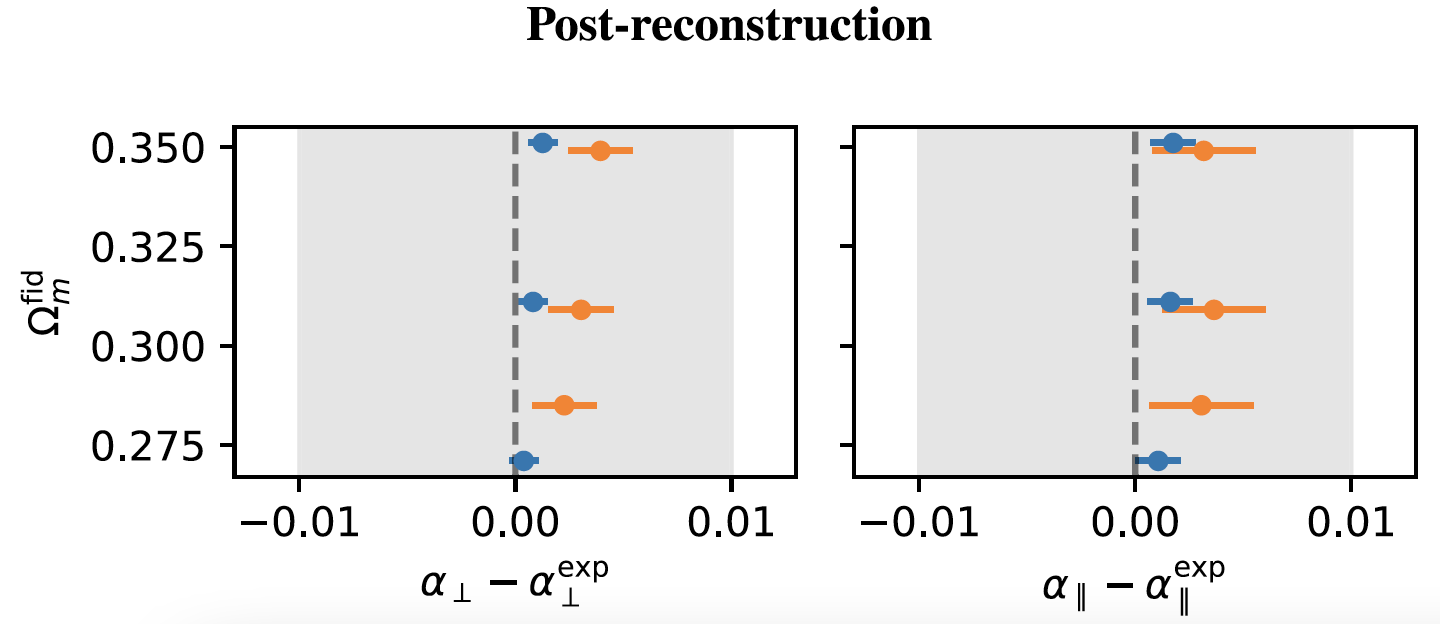
\includegraphics[width=0.49\textwidth]{fig/galaxies/bao_bias_postrecon.png}
    \caption{Impact of choice of fiducial cosmology in the recovered values
    of $\apara$ and $\aperp$ from BAO fits to the stacks of 1000 multipoles the \textsc{EZMOCKS} 
    (blue) and 84 \textsc{NSERIES} mocks (orange), for pre- (left panels) and post-reconstruction
    (right panels). Associated error bars correspond to the uncertainty estimated from 
    the mean of the mocks. The grey shaded areas correspond to 1 per cent shifts. 
    For comparison, the uncertainty on real data is 1.9 per cent for $\aperp$ 
    and 2.6 per cent for $\apara$ in the post-reconstruction case.
    }
    \label{fig:bao_bias_mocks}
\end{figure}

Another important test of our methodology consists in checking uncertainity estimation. 
With the sample of 1000 BAO measurements from mocks, we can study them statistically. 
Our uncertainties are derived by scanning the likelihood profile and finding the intervals
where the parameters $\aperp$ and $\apara$ increase the $\chi^2$ by 
unity\footnote{In the case marginalised errors in one parameter. For two parameters, 
the 68 and 95\% confidence intervals are defined by $\Delta \chi^2 = 2.3, \ 5.9$ respectively.} 
relative to its minimum. 
First, we compare the standard deviation of all best-fit values to the average uncertainty
found in all 1000 mocks. If uncertainties are correctly estimated then these two numbers 
match. Second, we could look at the pull distribution of each parameter $x_i$, defined as 
$Z_i \equiv (x_i - \bar{x}_i)/\sigma_{x_i}$. If the uncertainties are well behaved and Gaussian, 
then we should obtain $\bar{Z_i}=0$ and $\text{Var}(Z_i) = 1$. 
Table 6 in \cite{bautistaCompletedSDSSIVExtended2021} shows these statistics for BAO measurements. 
The results validate our methodology and we applied it to data.  

Figure~\ref{fig:eboss_dr16_lrg_bao} shows the best-fit correlation function model and 
the BAO constraints for the eBOSS DR16 LRG sample. 
Converting the constraints in $(\aperp,\apara)$ into ratios of distances, we obtained: 
\begin{equation}
    \mathbf{D}_{\text{ BAO},{\xi_\ell}} =
    \begin{pmatrix}
   D_M/r_d \\
   D_H/r_d 
    \end{pmatrix}=
    \begin{pmatrix}
     17.86 \pm 0.33 \\
     19.34 \pm 0.54 
     \end{pmatrix},
\end{equation}
which correspond to a BAO measurement at 1.9 per cent in the transverse direction 
and 2.8 per cent in the radial direction. 
Radial and transverse BAO measurements are correlated by -33\% for this dataset.  
These are the best constraints obtained from galaxies at redshifts above $0.6$.

\begin{figure} 
    \centering 
    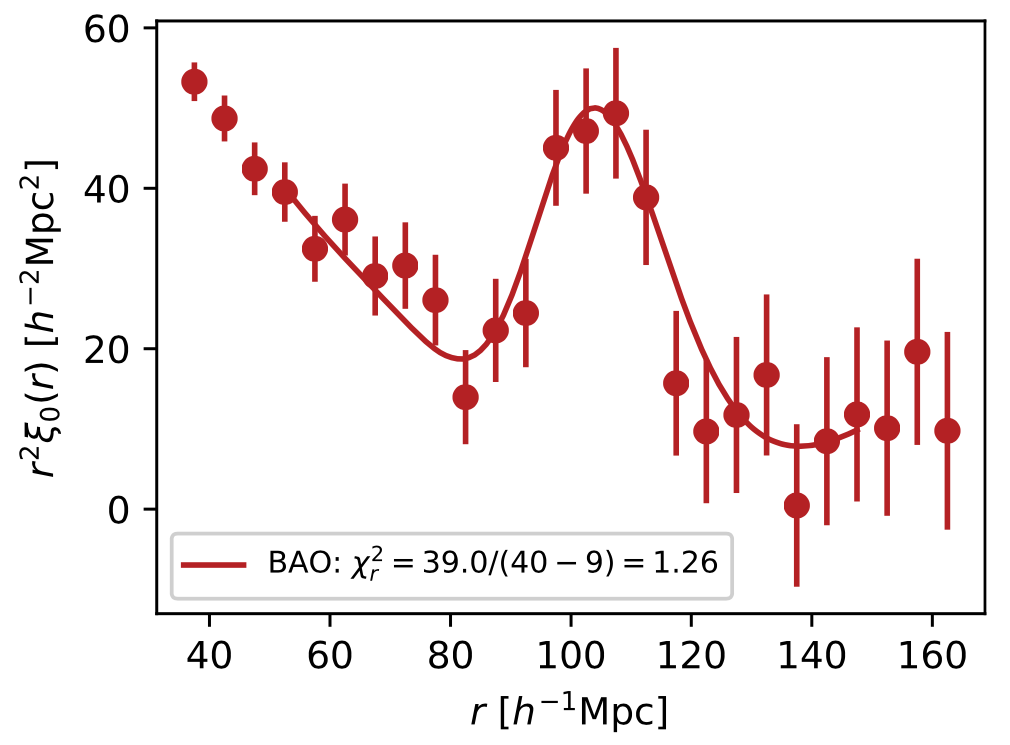
\includegraphics[width=0.33\textwidth]{fig/galaxies/eboss_dr16_lrg_bao_mono.png}
    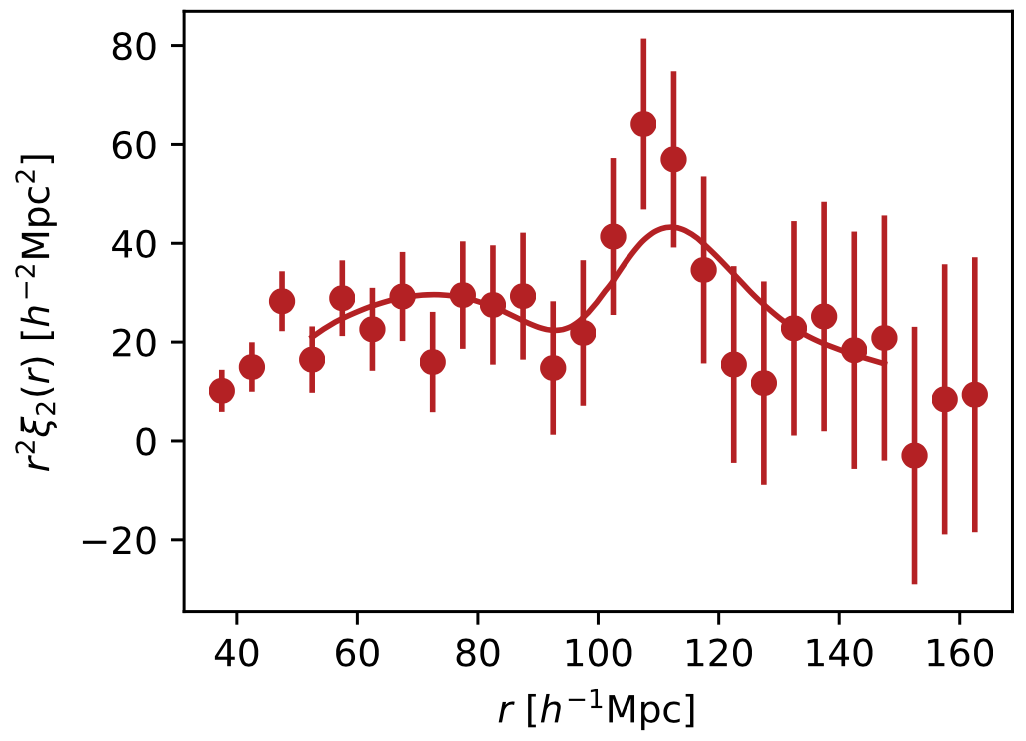
\includegraphics[width=0.33\textwidth]{fig/galaxies/eboss_dr16_lrg_bao_quad.png}
    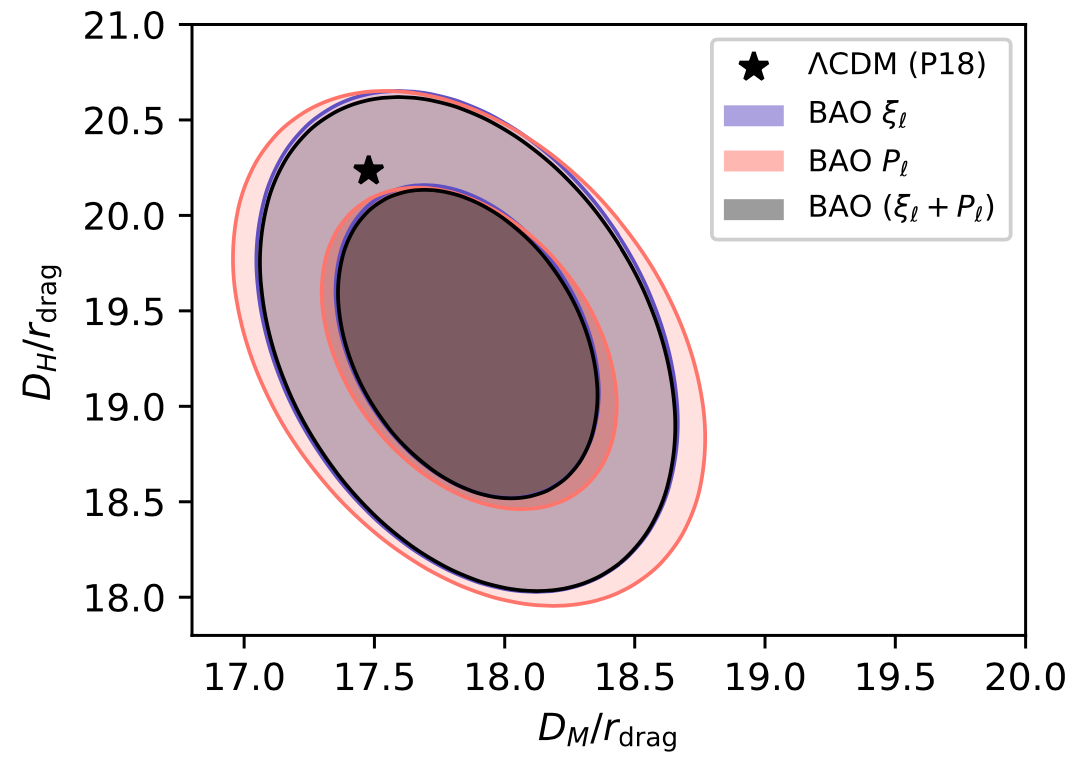
\includegraphics[width=0.33\textwidth]{fig/galaxies/eboss_dr16_lrg_bao_contours.png}
    \caption{Two left panels show the best-fit model for the correlation function monopole and 
    quadrupole for the reconstructed eBOSS LRG sample. The right panel shows the two-dimensional 
    constraints on the distance to sound horizon ratios, for the configuration and Fourier space 
    BAO analyses. The consensus BAO result is shown in grey. The star points to the prediction 
    of a flat $\Lambda$CDM model with Planck 2018 best-fit parameters. }
    \label{fig:eboss_dr16_lrg_bao}
\end{figure}

\section{Redshift-space distortions}
\label{galaxies:rsd}

The analysis of redshift-space distortions (RSD) aims to measure the growth-rate of structures $f$, 
as introduced in section~\ref{intro:probes:rsd}, by quantifying the anisotropies in the clustering 
of galaxies. As we seen before, assuming an incorrect fiducial cosmology when converting redshifts 
into distances also introduces anisotropies (the AP effect). Therefore in practice, an RSD analysis
yields simultaneously the combination $f(z)\sigma_8(z)$ and the distance ratios $D_H(z)/r_\text{drag}, D_M(z)/r_\text{drag}$. 

The main differences with respect to the BAO analysis (see previous section) is that the information 
about anisotropies come from the full shape of the two-point statistics, not only the peak. 
This complicates the RSD analysis in that we need to have accurate models for the full shape of 
the clustering down to some scale, and we cannot add empirical terms to be marginalised over as we did in the BAO analysis. 
Due to non-linearities of matter clustering and galaxy bias, it is increasingly hard to model scales below 
those well described by linear theory. For these midly non-linear scales, we need more advanced perturbation theory models. 
A huge variety of theoretical models have been developed in the past years (see \cite{bernardeauLargeScaleStructureUniverse2002}
for a review). 

In the analysis of eBOSS data, we used to types of models: 
the first one is based on regularised perturbation theory with second order bias and RSD correction terms
(\cite{taruyaBaryonAcousticOscillations2010, taruyaDirectFastCalculation2012}). We commonly refer to it as 
the \emph{TNS model}. The second one is based on convolution Lagrangian perturbation theory with Gaussian streaming
(\cite{carlsonConvolutionLagrangianPerturbation2013, wangAnalyticModelRedshiftspace2014}). We refer to it as 
the \emph{CLPT-GS model}. I implemented these models in python language in the package 
\textsc{baopy}\footnote{\url{https://baopy.readthedocs.io/}}. 

The TNS model is expressed as:
\begin{equation}
    P_g(k, \mu_k) = D_\text{FoG}(k, \mu_k) 
    \left[ 
        P_{g, \delta \delta}(k) + 2 f \mu_k^2 P_{g, \delta \theta}(k) + f^2 \mu_k^4 P_{\theta \theta}(k)
        + b_1^3 A(k, \mu_k, \beta) + b_1^4 B(k, \mu_k, \beta)
    \right],
    \label{eq:tns_model}
\end{equation}
where $b_1$ is the first order linear galaxy bias, $\beta \equiv f/b_1$, 
$(P_{g, \delta \delta}, P_{g, \delta \theta},P_{\theta \theta})$ are the non-linear isotropic galaxy 
auto power spectrum, galaxy-velocity divergence cross power spectrum and the velocity divergence auto power spectrum, respectively, 
which are themselves functions of first and second order bias parameters. These functions are provided by 
the RegPT scheme, implemented in \textsc{pyregpt}\footnote{\url{https://github.com/adematti/pyregpt}}.
The functions $A$ and $B$ are the RSD correction terms. The function $D_\text{FoG}$ can be either a Gaussian or a Lorentzian
of $k_\parallel = k\mu_k$
with characteristic scale $\sigma_\text{FoG}$ corresponding to the velocity dispersion on small scales. 
This model is computed in Fourier space, but it can be Fourier transformed to obtain a model in configuration space. 

The CLPT-GS model is uniquely defined in configuration space, and writtes as: 
\begin{equation}
 1 + \xi_{g,s}(\rperp, \rpara) = 
  \int  \frac{1}{\sqrt{2\pi \left[\sigma_{12}^2(r)+\sigma^2_\text{FoG}\right]}}
  \left[1+\xi_g(r)\right] 
  \exp{ - \frac{[r_\parallel-y-\mu v_{12}(r)]^2}
               {2\left[\sigma_{12}^2(r)+\sigma^2_\text{FoG}\right]}} dy
 %\begin{split}
 %   1+\xi_{\rm X}(r_\perp,r_\parallel)= & \int \frac{1}{\sqrt{2\pi \left[\sigma_{12}^2(r)+\sigma^2_{\rm FoG}\right]}}[1+\xi_{\rm X}(r)]\\
 %   & \times \exp{-\frac{[r_\parallel-y-\mu v_{12}(r)]^2}{2\left[\sigma_{12}^2(r)+\sigma^2_{\rm FoG}\right]}} dy,
 %   \end{split}
 \label{eq:clptgs_model}
\end{equation}
where $\xi_g(r)$, $v_{12}(r)$, and $\sigma_{12}(r)$ are obtained 
from CLPT and contains two bias terms. The dependency with $f$ is via a scaling of 
the functions $v_{12}, \sigma_{12}$ that are proportional to velocity. 
The integral corresponds to the convolution by velocities in the radial direction, 
characteristic of the Gaussian streaming formalism. 

Both the TNS and CLPT-GS models had to be tested agains n-body simulations. 
We were particularly interested in the scales of validity of these models 
for the case of the eBOSS LRG sample. Given the number of available realisations, 
we used the n-body suite of 84 realisations of \textsc{Nseries} simulations 
produced for the BOSS CMASS sample. We fitted the average correlation function 
of these simulations and measured the parameters $f\sigma_8, \aperp, \apara$. 
Figure~\ref{fig:rsd_bias_mocks} presents the results compared to expected values 
for both TNS and CLPT-GS models. The shaded green area shows the fiducial choice 
to be used in the data. 

\begin{figure}
    \centering 
    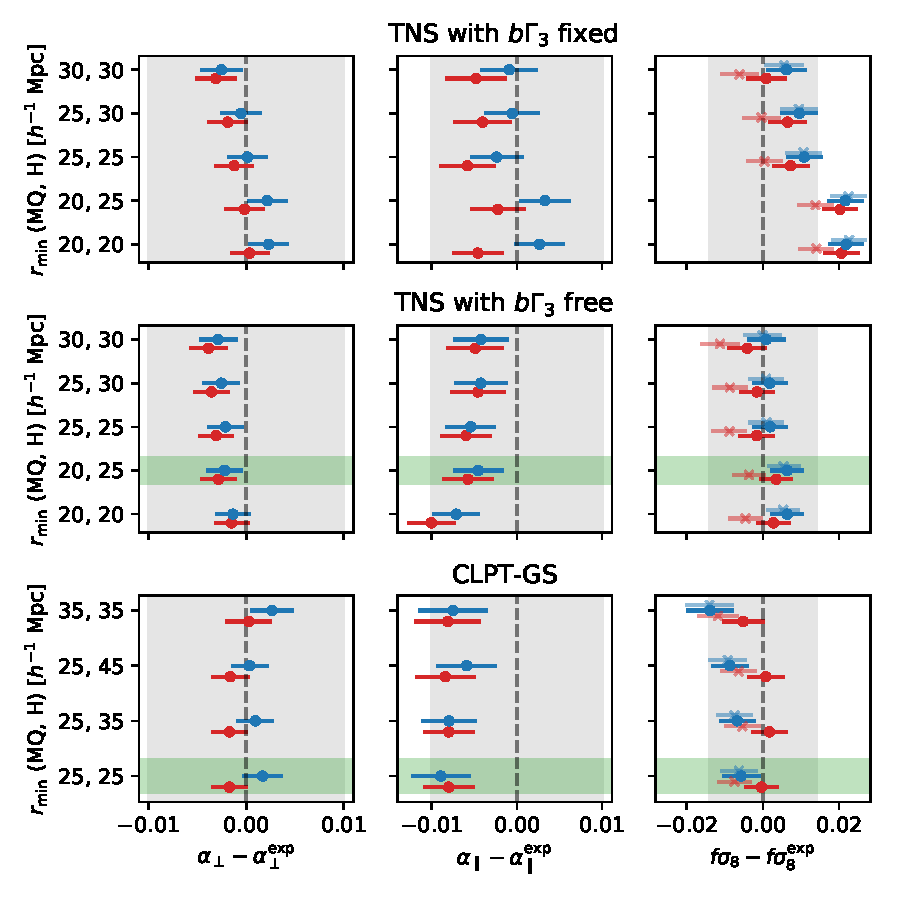
\includegraphics[width=0.7\textwidth]{fig/galaxies/rsd_rmin_nseries.pdf}
    \caption{Biases in the measurement of $f\sigma_8, \apara, \aperp$ obtained 
    from full-shape fits to the average of 84 multipoles from the \textsc{Nseries} 
    mocks as a function of the separation range used. 
    The y-axis displays the value of the minimal separation $r_\text{min}$ 
    used in fits of the monopole, quadrupole (MQ) and hexadecapole (H). 
    Top and mid rows display results for the TNS model when fixing or letting free 
    the bias parameter $b\Gamma_3$ respectively. 
    Bottom row presents results for the CLPT-GS model. 
    The blue circles correspond to the analysis using $\Omega_m^\text{fid} = 0.286$ 
    (the true value of simulations) while the red circles correspond to 
    $\Omega_m^\text{fid} = 0.31$. The crosses in the $f\sigma_8$ panels correspond 
    to their values before the scaling of $\sigma_8$ discussed in Figure~\ref{fig:rsd_fid_cosmo}. 
    The gray shaded areas correspond to 1 per cent errors in $\aperp, \apara$ and 
    to 3 per cent in $f\sigma_8$. 
    The green shared area shows our choice for baseline analysis for TNS and CLPT-GS models.}
    \label{fig:rsd_bias_mocks}
\end{figure}

Using the same simulations, we tested the dependency of our constraints to the choice of 
fiducial cosmology. Note that the fiducial cosmology enters twice in the modelling, first
when converting redshifts to distances; second, when computing the linear matter power spectrum 
template $P_m^\text{lin}(k)$, used as main ingredient for both models. 
Figure~\ref{fig:rsd_fid_cosmo} presents the results for three choices of fiducial cosmology. 
While for $\aperp, \apara$ the biases or trends are negligible, $f\sigma_8$ shows 
a strong dependency with $\Omega_m^\text{fid}$, shown as crosses in the figure. 
This dependency is mainly caused by the assumed $\sigma_8$ value, that corresponds to the 
one derived from the fiducial $P_m^\text{lin}(k)$ via Eq.~\ref{eq:variance_linear_field_smoothed}.
The resulting $f$ of the fit is scaled by this $\sigma_8$. 
We can reduce this dependency by recomputing $\sigma_8$ using $R=8\alpha$\hmpc,
where $\alpha \equiv \aperp^(2/3)\apara^(1/3)$ is the isotropic dilation factor obtained from the best-fit $\aperp,\apara$.
In effect, this keeps the scale at which $\sigma_8$ is fitted fixed relative 
to the data in units of $h^{-1}$Mpc, which only depends on $\Omega_m^\text{fid}$. 
This is an alternative approach to the recently proposed $\sigma_{12}$ parametrisation 
(\cite{sanchezArgumentsUsingMpc2020}), where the radius of the top-hat function is set to 
$R=12$~Mpc (in units of Mpc) instead of $R=8$\hmpc (in units of \hmpc). 
The circles in the right panel of Figure~\ref{fig:rsd_fid_cosmo} shows the results with 
the recomputed $\sigma_8$ for each case, showing that this procedure indeed reduces the 
trend of $f\sigma_8$ with $\Omega_m^\text{fid}$. 
This topic is also discussed in Appendix A of \cite{alamCompletedSDSSIVExtended2021}. 

\begin{figure}
    \centering 
    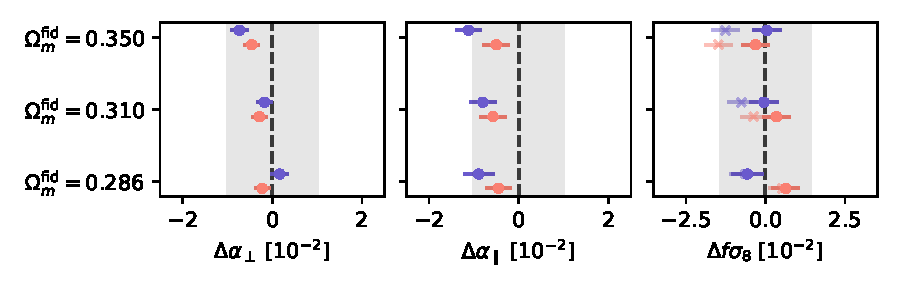
\includegraphics[width=0.6\textwidth]{fig/galaxies/rsd_nseries_fidcosmo_updated.pdf}
    \caption{Biases in best-fit parameters for both CLPT-GS (blue) and TNS (red) 
    models from fits to the average multipoles of 84 \textsc{Nseries} mocks.
    Shaded grey areas show the equivalent of 1 per cent error for $\aperp,\apara$
    and 3 per cent for $f\sigma_8$. In the right panel, crosses indicate $f\sigma_8$ values
    when $\sigma_8$ is not recomputed as described in the text. 
    The true cosmology of the mocks is $\Omega_m = 0.286$. 
    For reference, the errors on our data sample are $\sim$ 2, 3 and 10 per cent for 
    $\aperp, \apara, f\sigma_8$ respectively. }
    \label{fig:rsd_fid_cosmo}
\end{figure}

After validating the model, we tested the impact of different halo occupation distribution (HOD) models 
and observational effects, both introduced in simulations. We found that none of these modifications 
introduces significant biases our contraints of $(f\sigma_8, \aperp, \apara)$, though the shifts we observe 
were added as systematic uncertainties in quadrature to the statistical ones. 
Table 10 of \cite{bautistaCompletedSDSSIVExtended2021} summarises the systematic errors which are assumed to be
diagonal (no covariance between the three parameters) for simplicity. For our RSD analysis, 
systematic errors are about half of the statistical ones for $f\sigma_8$ and slightly less for $\aperp, \apara$. 
In quadrature, final uncertainties increase by up to 20\% due to systematic errors. 

We also attempted to analyse our biases and uncertainties statistically with the set of 1000 \textsc{EZmocks}. 
However, an important caveat is that these mocks only solve approximatively the clustering, and therefore are not 
the better suited to test RSD fitting. We proceeded to fit the 1000 realisations and we compared 
the average uncertainty to the standard deviation of best-fit parameters among all mocks. These numbers 
agree sufficiently well, particularly for $f\sigma_8$. The pull distributions of each parameters do not 
point to any under/over estimation of uncertainties.  

Figure~\ref{fig:eboss_dr16_lrg_rsd_bestfit} presents the best-fit TNS and CLPT-GS models to the correlation function 
multipoles of the eBOSS DR16 LRG sample. 
Both models are basically indistinguishable even though their are derived differently. The constraints are also 
similar between the two models, so we combined them into a single results by averaging their best-fit parameters 
and their covariances. 
Figure~\ref{fig:eboss_dr16_lrg_rsd_contours} show the final constraints on $f\sigma_8$ and the distance ratios, 
compared to the same analysis in Fourier space. We also show the consensus result computed using the method 
by \cite{sanchezClusteringGalaxiesCompleted2017a}, which assumes Gaussianity of each posterior distribution 
(see the next section for a further discussion). 
The final RSD constraints from the correlation function fits are:
\begin{equation}
    \mathbf{D}_{\text{RSD}, {\xi_\ell}} =  
    \begin{pmatrix}
   D_M/r_d \\
   D_H/r_d \\
   f\sigma_8 
    \end{pmatrix}=
    \begin{pmatrix}
    17.42 \pm 0.40 \\
    20.46 \pm 0.70 \\
    0.460 \pm 0.050
    \end{pmatrix}
\end{equation}
which correspond to a 11\% measurement of $f\sigma_8$ at $z_\text{eff} = 0.7$. 
This uncertainty is slightly reduced when combining with the Fourier space results 
and with BAO results from the previous section. 
The combination between Fourier and configuration space results
will be discussed in the following section. 

\begin{figure}
    \centering
    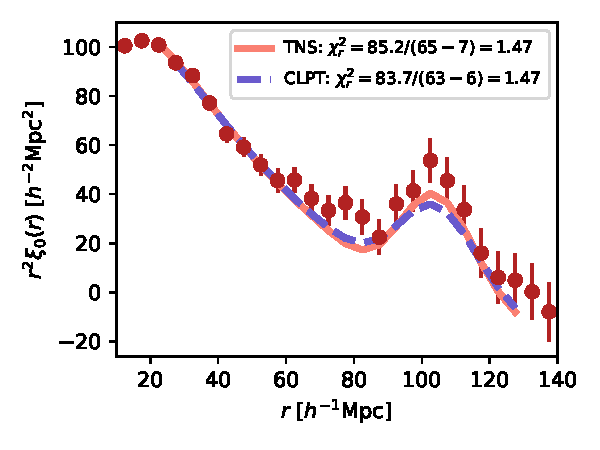
\includegraphics[width=0.33\textwidth]{fig/galaxies/DR16_LRG_RSD_v7_2_bestfits_mono.pdf}
    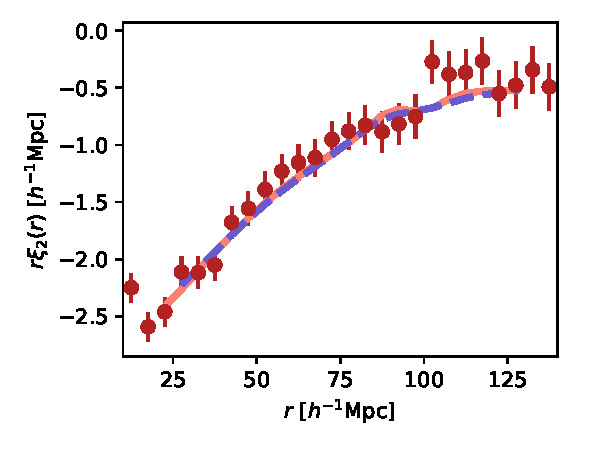
\includegraphics[width=0.33\textwidth]{fig/galaxies/DR16_LRG_RSD_v7_2_bestfits_quad_scaler1.pdf}
    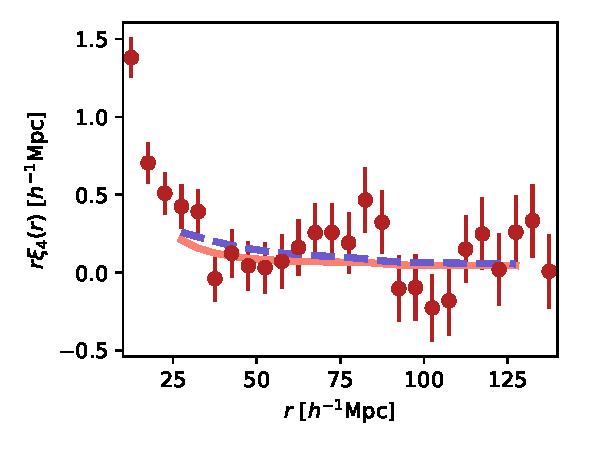
\includegraphics[width=0.33\textwidth]{fig/galaxies/DR16_LRG_RSD_v7_2_bestfits_hexa_scaler1.pdf}
    \caption{Best-fits models of redshift-space distortions (RSD) to the 
    eBOSS DR16 LRG multipoles. 
    Left, mid and right panel display mono, quad and hexadecapole, respectively. 
    Note that only the monopole is scaled by $r^2$ while the others are scaled by $r$.
    The CLPT-GS model is shown by the blue dashed line while the TNS
    model is shown by the red solid line. 
    }
    \label{fig:eboss_dr16_lrg_rsd_bestfit}
\end{figure}


\begin{figure}
    \centering
    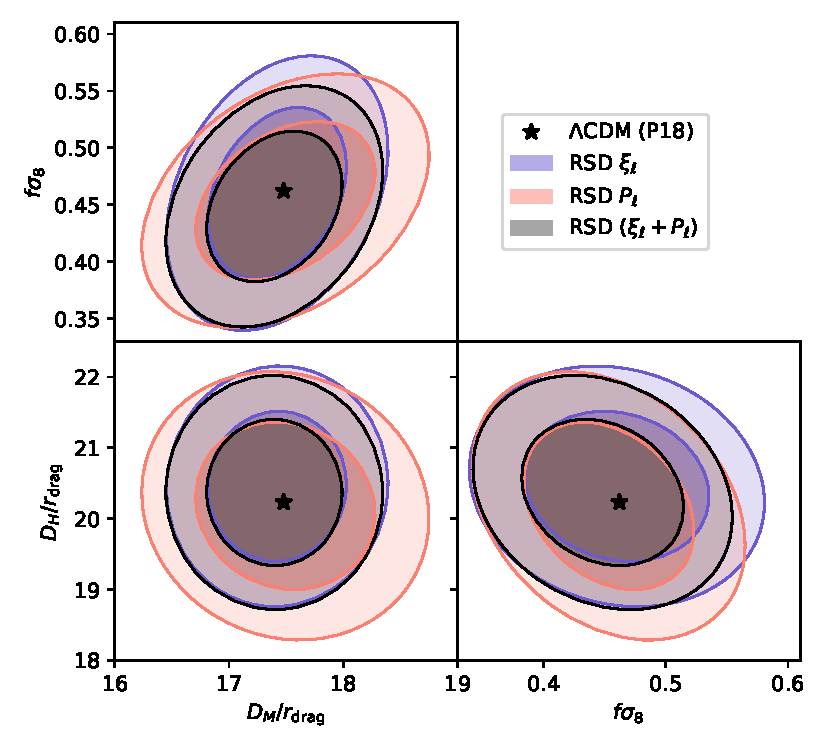
\includegraphics[width=0.5\textwidth]{fig/galaxies/DR16_LRG_consensus_rsd_planck.pdf}
    \caption{Constraints on $D_M/r_d, D_H/r_d$ and $f\sigma_8$ $z_\text{eff} = 0.7$ 
    from the full-shape 
    RSD analysis of the completed eBOSS LRG sample.
    Contours show 68 and 95 per cent confidence regions for the analyses in 
    configuration space (blue), Fourier space (red) 
    and the combined (grey). 
    The expected values in a flat $\Lambda$CDM 
    model with best-fit parameters from Planck 2018 results 
    is indicated as a black star.}
    \label{fig:eboss_dr16_lrg_rsd_contours}
\end{figure}



\section{Joint clustering analysis in Fourier and Configuration space}
\label{galaxies:joint}

From the same catalogue of angular positions and redshifts, we can perform 
two different clustering analyses: one in Fourier space (FS) and the other in 
Configuration space (CS). How to define a consensus result from both analysis 
which might yield slightly different results? In this section I expose the work 
lead by my PhD students Tyann Dumerchat and Vincenzo Aronica on how to combine  
BAO and RSD constraints from both spaces into a single consensus result. 

\cite{sanchezClusteringGalaxiesCompleted2017a} proposed a method to combine
two correlated Gaussian posteriors into a single one. I refer to it as the 
Gaussian approximation (GA) method. The GA method was used in 
BOSS (\cite{alamClusteringGalaxiesCompleted2017}) and it was slightly improved 
in eBOSS (\cite{bautistaCompletedSDSSIVExtended2021}). 
The main idea is that we want to combine a set of vectors containing the best-fit 
parameters of different analysis (and their respective error matrix) into a single vector 
of parameters and a single error matrix. 
For example in BOSS and eBOSS, we aimed at combining 
the vectors $\vec{p} \equiv {f\sigma_8, \aperp, \apara}$ obtained from FS and CS analyses. 
The GA method uses an estimate the correlations between $\vec{p}_\text{FS}$ and $\vec{p}_\text{CS}$,
and built a large covariance matrix used to combine the vectors and error matrices. 
Currently the best method to obtain these correlations between FS and CS results is using mock catalogues.
This provides with an estimate of a sort of ``ensemble averaged'' correlations (though limited by the 
number of realisations). However, the real data is a single realisation of the ensemble, and 
the correlations between FS and CS are also suceptible to fluctuate, just as the individual parameters 
and their uncertainties. In \cite{bautistaCompletedSDSSIVExtended2021} we developed 
a method to account for this fact, where we adjust the correlations for each realisation based on 
the vectors $\vec{p}$ and their error matrices of that particular realisation. 

In \cite{dumerchatBaryonAcousticOscillations2022}, we developed an analysis where we fit jointly 
the correlation function and power spectrum while accounting for their covariance.
I refer to it as the joint space (JS) method.  
The covariance is built at the multipole level, using a set of mock catalogues.
Figure~\ref{fig:covariance_ezmock} shows the correlation coefficients of CS and FS multipoles, 
including the cross-correlation terms. The wiggles observed in the cross-correlation terms 
can be simply explained by the fact that CS and FS are related via Hankel transforms 
(see Appendix A of \cite{dumerchatBaryonAcousticOscillations2022} for an explicit derivation). 
We tested and validated this framework on the BAO analysis of the eBOSS LRG sample 
(section~\ref{galaxies:bao}) where we fit for a single $\aperp$ and $\apara$, though 
amplitudes of power-laws are independent for each space. 
The main advantage of the JS method is that we do not assume Gaussian posteriors at the parameter level, 
only at the multipole level when fitting our model (which is quite common assumption). 
The posteriors on the resulting $(\aperp, \apara)$ can also be non-Gaussian. 
Figure~\ref{fig:non_gaussian_contours} displays few examples from BAO fits to mock realisations where 
the CS and FS posteriors are Gaussian (left) or non-Gaussian (right panels), 
and the resulting combination from GA and JS methods. 
For the non-Gaussian cases, the GA method fails to correctly describe the posterior, 
underestimating uncertainties. 


\begin{figure}
    \centering
    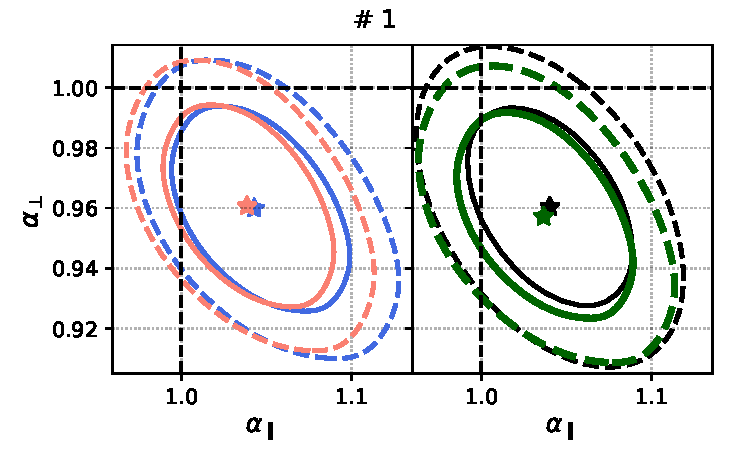
\includegraphics[width=0.45\textwidth]{fig/galaxies/gaussian_contours0.pdf}  
    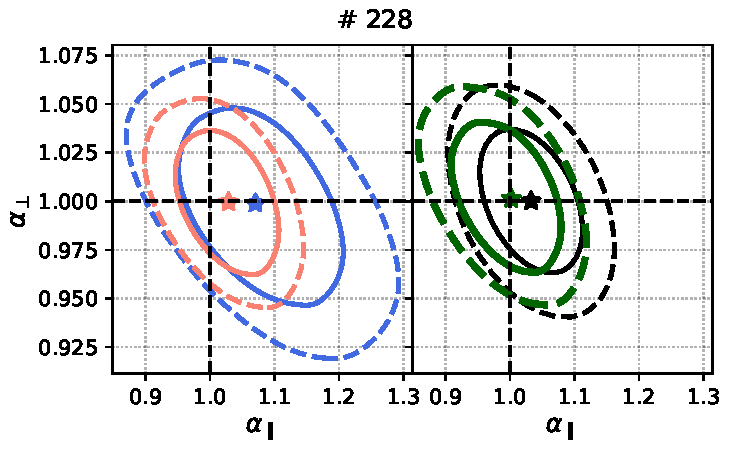
\includegraphics[width=0.45\textwidth]{fig/galaxies/non_gaussian_contours1.pdf}  
    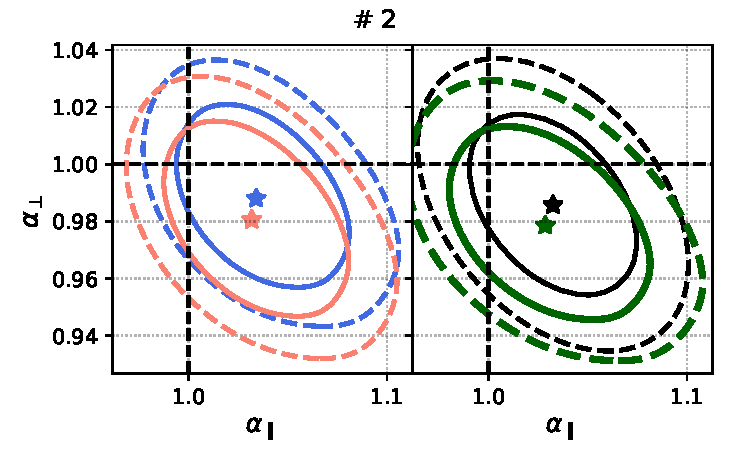
\includegraphics[width=0.45\textwidth]{fig/galaxies/gaussian_contours1.pdf}  
    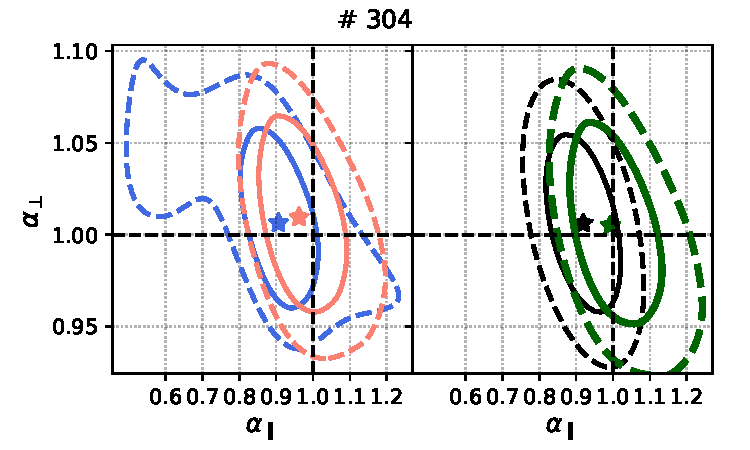
\includegraphics[width=0.45\textwidth]{fig/galaxies/non_gaussian_contours2.pdf}  
    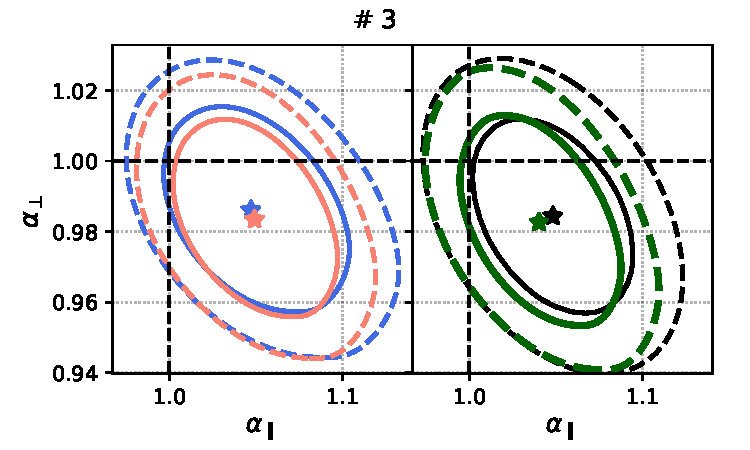
\includegraphics[width=0.45\textwidth]{fig/galaxies/gaussian_contours2.pdf}  
    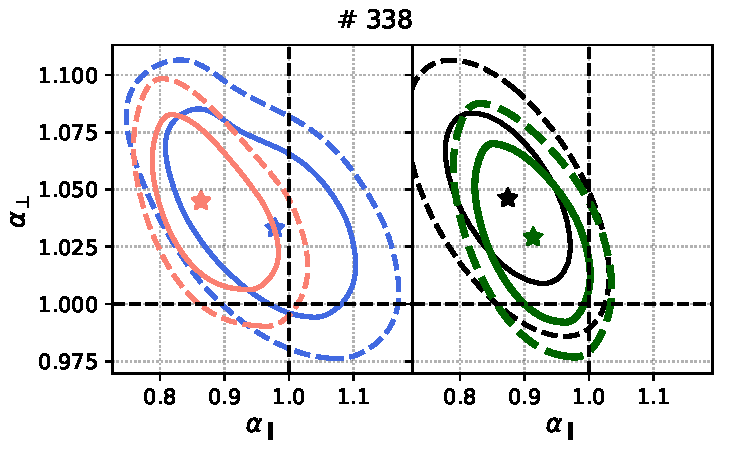
\includegraphics[width=0.45\textwidth]{fig/galaxies/non_gaussian_contours3.pdf}  
  \caption{Posteriors on the BAO fits of some \textsc{EZmocks} realisations 
  realisations. We display cases where contours found in 
  configuration or Fourier space are Gaussian (left) and non Gaussian(right). 
  Red contours are for Fourier space (FS), blue for configuration space (CS), 
  black for the Gaussian approximation (GA) and green for the joint space (JS) fits.  
  The expected value is the intersection of the dotted black lines,
  and the best fit values are described by a star for the JS and GA methods. 
  We can see how the JS method yields better combined results that are not necessarily Gaussian.
  Extracted from \cite{dumerchatBaryonAcousticOscillations2022}. 
  }
  \label{fig:non_gaussian_contours}
  \end{figure}

Vincenzo Aronica is currenlty working on the application of joint space analysis 
for the case of redshift-space distortions (RSD). 
He implemented the TNS model (section~\ref{galaxies:clustering:eboss_dr16_lrgs}) 
in Fourier and configuration space in the \textsc{baopy} package. 
The tests on the suite of 84 realisations of \textsc{nseries} n-body simulations are 
promising, though there are some subtleties to solve related to the relative normalisation 
(or linear bias) amplitudes between FS and CS. Currently we use the same values of biases 
for both space, in addition to $\aperp, \apara, f\sigma_8$. 
Vincenzo will recompute power spectra for a given set of mock 
catalogues using a consistent normalisation and window function calculations provided by 
\textsc{pypower}. 

The work on BAO and RSD joint fits in Fourier and configuration space 
will be discussed and hopefully applied to the analysis of DESI data. 


\section{Cross-correlation with radio surveys}
\label{galaxies:radio}

The study of large-scale structures will soon be improved thanks to 
observations of the distribution of neutral hydrogen (HI) via the emission 
of photons from the 21cm hyperfine transition of the electron. 
Future 21cm surveys such as the Square Kilometer Array (SKA) will be able to 
observe the Universe with intensity mapping up to redshifts of 3, 
opening an alternate window to that provided by spectroscopic surveys. 
The term \emph{intensity mapping} refers to the fact that we measure 
the integrated flux from unresolved sources at a given location in space.

During my postdoctoral stay at the University of Portsmouth, 
I contributed to the study of a currently available 21cm survey produced by the Green Bank Telescope (GBT).
I was particularly interested in the study of cross-correlations between the 21cm 
observed by GBT and the eBOSS galaxies observed in the same volume. 
With the cross-correlation function we could infer the product of the average neutral hydrogen fraction 
$\Omega_\text{HI}$ at redshift $z_\text{eff} = 0.8$ with the bias of HI $b_\text{HI}$.  
These parameters are important ingredients for models of clustering of the 21cm emission.
I overview the main findings of this work in this section but further details 
are described in \cite{wolzConstraintsCrosscorrelationEBOSS2022}. 

The use of 21cm intensity mapping to measure the large-scale structures has been 
extensively studied theoretically 
(\cite{bharadwajUsingHIProbe2001,
battyeNeutralHydrogenSurveys2004,
mcquinnCosmologicalParameterEstimation2006,
changBaryonAcousticOscillation2008a}) 
and with simulations 
(\cite{mesinger21CMFASTFastSeminumerical2011,
villaescusa-navarroIngredients21Cm2018} and references therein). 
On large scales, 21cm flux fluctuations trace those of dark matter density, while on smaller scales 
the physics of the gas and its connection to halos complexifies the modelling.  
Including redshift-space distortions, a linear model for the 21cm power spectrum is essentially the 
same as the linear model for galaxy clustering. 
In \cite{villaescusa-navarroIngredients21Cm2018}, an extensive study using the IllustrisTNG 
n-body hydro simulation quantified several ingredients commonly used in more complex models of 
the 21cm power spectra, such as the HI content of halos, the HI probability density function, 
the HI bias with respect to matter and others. 

The data sets we used in our study were
the eBOSS luminous red galaxy (LRG) and emission line galaxy (ELG) samples in one hand, 
and the Green Bank Telescope (GBT) 21cm maps in the other hand.
The eBOSS LRG sample is already described in section~\ref{galaxies:catalogue} while the
ELG sample is described in \cite{raichoorCompletedSDSSIVExtended2020}. 
The GBT maps are observations of a 100 deg$^2$ patch of sky at frequencies from 700 to 900 MHz divided into 256 channels, 
corresponding to HI emission between $0.6 < z < 1.0$, perfectly overlapping with our galaxy samples in area and redshift. 
The angular resolution of HI observations varies from 0.31 deg at 700 MHz to 0.25 deg at 900 MHz. 
In order to reduce the impact of varying PSF, all channels are convolved by an artificial beam of 0.44 deg. 
The maps we used are an extension to those produced by \cite{masuiMeasurement21Cm2013}, including extra scans
which increase the area and depth. 
The raw data is contaminated by radio frequency interference and some channels are therefore masked. 
Foregrounds are removed with a technique named \emph{FastICA}, which stands for fast independent 
component analysis. I was provided several maps with different number of foreground components removed.
Once the final area of GBT maps was fixed, I cut the eBOSS LRG and ELG samples to the same area. 
Figure~\ref{fig:gbt_footprint} shows a redshift slice (or one channel) of the foreground-cleaned GBT HI map
and the LRG and ELG angular distribution in the same patch of sky. 

\begin{figure}
    \centering 
    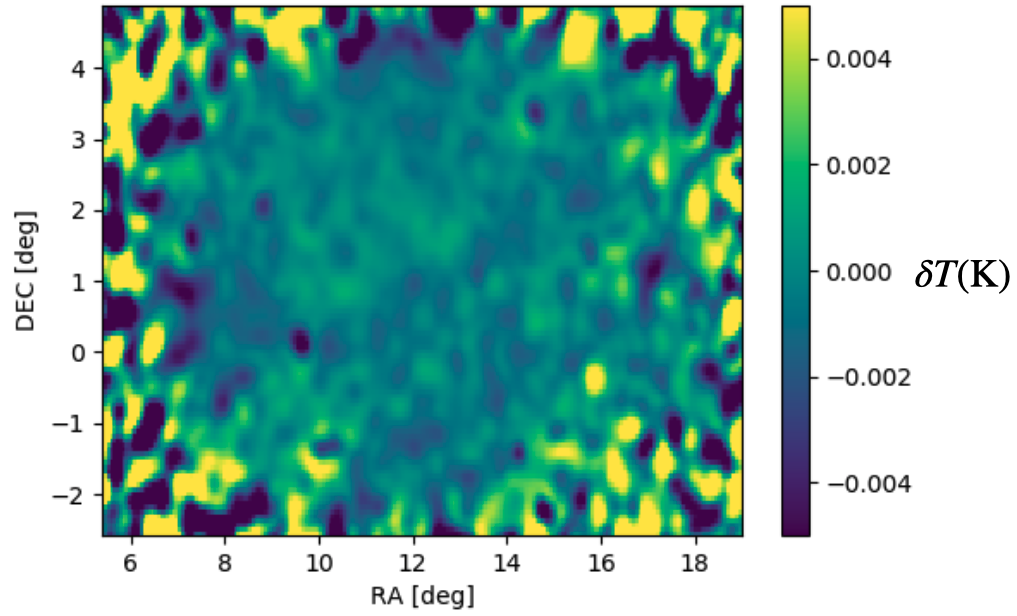
\includegraphics[width=0.6\textwidth]{fig/galaxies/gbt_map.png}
    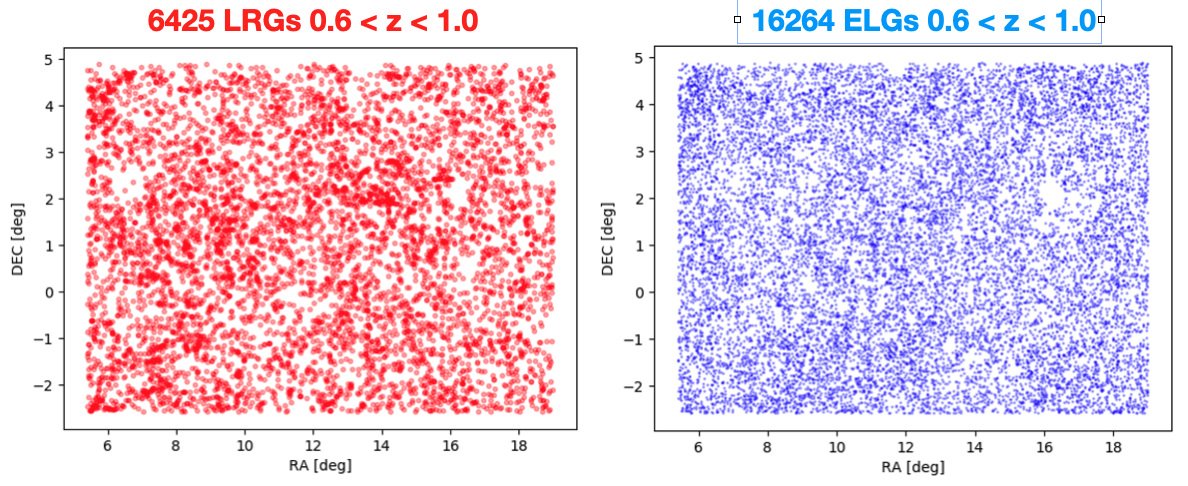
\includegraphics[width=\textwidth]{fig/galaxies/gbt_eboss_galaxies.png}
    \caption{Top panel: a redshift slice of the 21cm HI map from the Green Bank Telescope after foreground removal. 
    Bottom panels: the angular distribution of all eBOSS LRGs and ELGs falling in the same sky area. }
    \label{fig:gbt_footprint}
\end{figure}

The cross-correlations between eBOSS galaxies and 21cm temperature maps was computed 
in Fourier space by \cite{wolzConstraintsCrosscorrelationEBOSS2022} and in configuration space by me. 
The cross-correlation estimator I used is the same used for the quasar-\lya forest cross-correlation 
described in section~\ref{forests:bao:correlations}, which assumes that galaxies (in this case)
are shot-noise dominated and that voxels of the 21cm map are independent. These assumptions are 
not quite valid for our sample but I left further developments for future work. 
For instance, one could perfom 
the study of cross-correlations with a maximum likelihood method 
(see e.g. section~\ref{velocities:maximum_likelihood}) or in Fourier space but correctly accounting for 
the convolution by the window function of these surveys, which was not explicitly done in 
\cite{wolzConstraintsCrosscorrelationEBOSS2022}.

Figure~\ref{fig:gbt_cross_correlation} displays the monopoles and quadrupoles of the cross-correlation function 
between 21cm temperature fluctuations and eBOSS galaxies. Both ELG and LRG show non-zero correlations with the 
temperature maps that extend to cosmological scales. 
In particular, we clearly see a non-zero quadrupole, which was measured for the first time in this analysis.  
The covariance matrix of the multipoles was computed with the jacknife technique, 
using 96 independent subsets of the data. Due to the estimator I used, neighbouring separation bins in the 
monopole are strongly correlated. 

\begin{figure}
    \centering 
    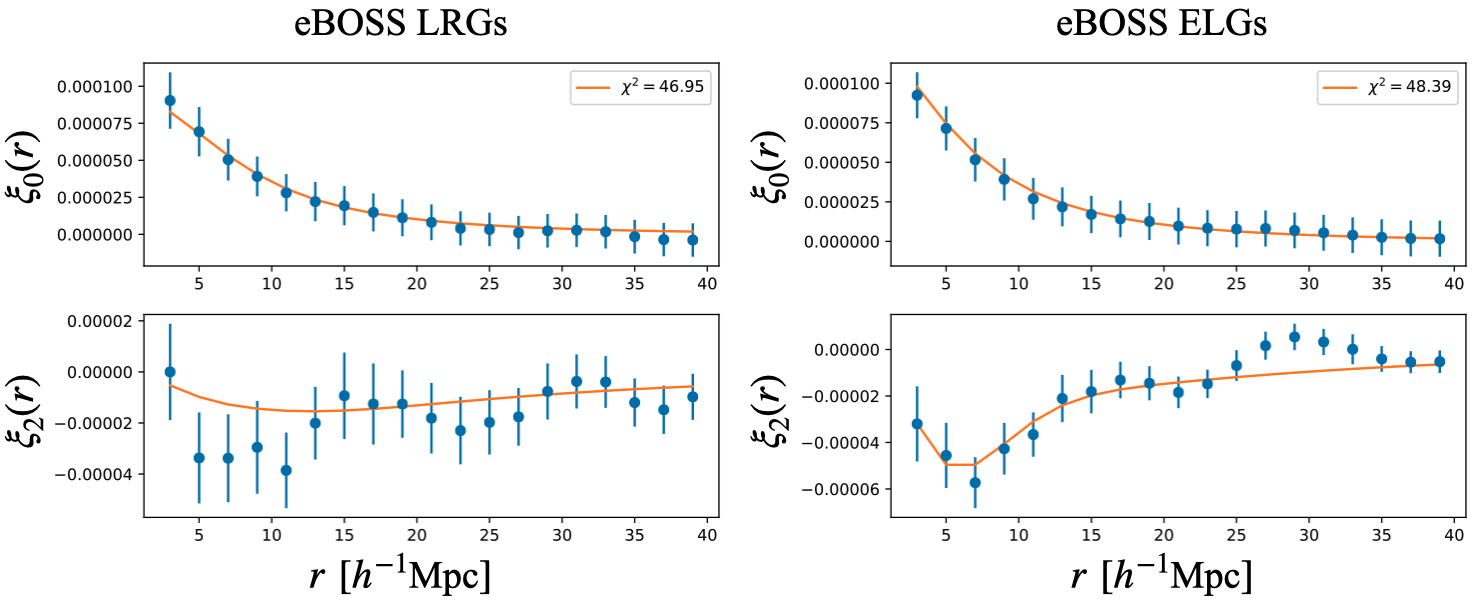
\includegraphics[width=\textwidth]{fig/galaxies/gbt_mono_quad.png}
    \caption{Cross-correlation function multipoles between 21cm temperature fluctuation maps from the Green Bank Telescope 
    and the eBOSS samples of Luminous Red Galaxies (left) and Emission Line Galaxies (right). 
    Uncertainties are computed with jacknife resampling and solid lines correspond to the best-fit models. 
    }
    \label{fig:gbt_cross_correlation}
\end{figure}

I attempted to fit the temperature-galaxy cross-correlation with the following model:  
\begin{equation}
    P(k, \mu) = \frac{b_\text{gal}b_\text{ HI}\bar{T}_\text{ HI}}
                     {(1+k^2\mu^2\Sigma_\text{FoG}^2)^2}
                (1+\beta_\text{gal}\mu^2)(1+\beta_\text{HI}\mu^2)P_\text{lin}(k)e^{-k^2 R_\text{beam}^2(1-\mu^2)/2}
    \label{eq:model_hi_gal}
\end{equation}
which includes a term for Fingers-of-God with dispersion $\Sigma_\text{FoG}$,
and a damping in the transverse (angular) direction to account for the effect of the beam of the GBT instrument, with 
characteristic scale $R_\text{beam}$. 
The solid lines in Figure~\ref{fig:gbt_cross_correlation} show the best-fit models, which have in total 6 free parameters. 
The $\chi^2$ values are also shown in the figure, which correspond to 30 data points (24 degrees of freedom). 
The fits are generally well behaved. 
I do not show values for the best-fit parameters and their uncertainties because of the caveats I mentioned before
related to the estimator and the covariance matrices. Also at the time of my analysis, we did not have mock catalogues 
to test my methodology.  

\cite{wolzConstraintsCrosscorrelationEBOSS2022} proceeded with the analysis of the cross power spectrum monopole
and fitted for the amplitude of the signal, after testing our methods on mock catalogues. 
Using different scale ranges, we obtained constraints on the combination $\Omega_\text{HI}b_\text{HI}r$ at $z_\text{eff}=0.8$,
where $r$ is an empirical cross-correlation term that depends on the galaxy sample. 
Table 1 of \cite{wolzConstraintsCrosscorrelationEBOSS2022} summarises results. For instance, 
for conservative choices for the analysis, we find $\Omega_\text{HI}b_\text{HI}r = (0.48\pm0.12)\times 10^{-3}$ for GBT x ELGs 
and $(0.38\pm0.12)\times 10^{-3}$ for GBT x LRGs, corresponding to 5 and 4.2$\sigma$ detections respectively. 

This work is on the pathway for precision measurements with future 21cm surveys such as SKA 
(\cite{squarekilometrearraycosmologyscienceworkinggroupCosmologyPhaseSquare2020}).

